\chapter{Thermodynamic modeling of the Pd-Zn-M system and its implication to tailor catalysts} \label{chap:intermetallics}

\section{Introduction} \label{intermetallics:sec:intro}

\section{Thermodynamic modeling of the Pd-Zn system with uncertainty \\quantification} \label{intermetallics:sec:PdZn}
Pd–Zn intermetallic catalysts show encouraging combinations of activity and selectivity on well-defined active site ensembles \cite{Dasgupta2022}. Thermodynamic description of the Pd–Zn system, delineating phase boundaries and enumerating site occupancies within intermediate alloy phases, is essential to determining the ensembles of Pd–Zn atoms as a function of composition and temperature. 

Combining the present extensive first-principles calculations and available experimental data, the Pd–Zn system was remodeled using the CALculation of PHAse Diagrams (CALPHAD) approach. High throughput modeling tools with uncertainty quantification, i.e., ESPEI and PyCalphad, were incorporated in the phase analysis. The site occupancies across the $\gamma$ phase composition region were given special attention. A four-sublattice model was used for the $\gamma$ phase owing to its four Wyckoff positions, i.e., the outer tetrahedral (OT) site 8c, the inner tetrahedral (IT) site 8c, the octahedral (OH) site 12e, and the cuboctahedral (CO) site 24g. The site fractions of Pd and Zn calculated from the present thermodynamic model show the occupancy preference of Pd in the OT and OH sublattices in agreement with experimental observations. The force constants obtained from DFT-based phonon calculations further support the tendency of Pd to occupy the OH sublattice compared with the IT and CO sublattice. The catalytic ensembles changing from Pd monomers (Pd1) to trimers (Pd3) on the $\gamma$ phase surface are attributed to the increasing Pd occupancy in the OH sublattice.

\subsection{Modeling details} \label{intermetallics:ssec:PdZnmodel}
%%% Phase information and Gibbs energy models
The Pd–Zn system contains 6 solution phases, i.e., Liquid, FCC, HCP, BCC$\_$B2($\beta$), FCC$\_$L1$_0$ ($\beta_1$), and Gamma ($\gamma$), and 3 stoichiometric compounds, i.e., Pd$_2$Zn, PdZn$_2$, and Pd$_9$Zn$_{91}$ based on the works summarized by Vizdal et al. \cite{vizdal2006experimental}. Details of these phases can be seen in Table \ref{intermetallics:PdZn_phases}, including phase names, crystallographic information, and the sublattice models of phases used in the present work.

\begin{table}[H]
    \footnotesize
    \centering
    \caption{Crystallographic information for phases in the Pd–Zn system and their sublattice models used in the present CALPHAD modeling.}
    \begin{tabular}{>{\raggedright\arraybackslash}m{2.5cm}>{\raggedright\arraybackslash}m{2.5cm}>{\raggedright\arraybackslash}m{2cm}>{\raggedright\arraybackslash}m{2.5cm}>{\raggedright\arraybackslash}m{6cm}}
        \hline
         \textbf{Phase name} & \textbf{Strukturbericht} & \textbf{Space group} & \textbf{Pearson symbol} & \textbf{Model} \\
        \hline
         Liquid($L$) &  &  &  & (Pd,Zn)$_1$ \\
         FCC$\_$A1 & A1 & $Fm\Bar{3}m$ & cF4 & (Pd,Zn)$_1$ \\
         HCP$\_$Zn & A3 & $P6_3/mmc$ & hP2 & (Pd,Zn)$_1$ \\
         BCC$\_$A2 & A2 & $Im\Bar{3}m$ & cI2 & (Pd,Zn)$_1$ \\
         BCC$\_$B2 ($\beta$) & B2 & $Pm\Bar{3}m$ & cP2 & (Pd,Zn)$_{0.5}$(Pd,Zn)$_{0.5}$ \\
         FCC$\_$L1$_0$($\beta_1$) & L1$_0$ & $P4/mmm$ & tP2 & (Pd,Zn)$_1$(Pd,Zn)$_1$ \\
         Gamma ($\gamma$) & D8$_2$ & $I4\Bar{3}m$ & cI52 & (Pd,Zn)$_2$(Pd,Zn)$_3$(Pd,Zn)$_2$(Pd,Zn)$_6$ \\
         Pd$_2$Zn &  & $Pnma$ & oP12(C23) & (Pd)$_2$(Zn)$_1$ \\
         PdZn$_2$ &  & $Cmm2$ & oS48 & (Pd)$_1$(Zn)$_2$ \\
         Pd$_9$Zn$_{91}$ &  &  &  & (Pd)$_{0.09}$(Zn)$_{0.91}$ \\
        \hline
    \end{tabular}
    \label{intermetallics:PdZn_phases}
\end{table}

Phase equilibrium properties of the Pd–Zn system published before 2006 were reviewed by Vizdal et al. \cite{vizdal2006experimental}. Massalski \cite{massalski1986binary} reported the solubility of Zn in FCC to be about mole fraction of Zn $x_{Zn}$ = $0.18 - 0.20$, and similar values were also observed by Hansen and Anderko \cite{hansen1958constitution}. The maximum solubility of Zn in FCC was around $x_{Zn}$ = $0.26$ at 1000 reported by Chiang et al. \cite{ChiangIpserChang1977} and Kou and Chang \cite{kou1975thermodynamics}. The solubility of Pd in HCP was reported to be lower than $x_{Zn}$ = 0.01 \cite{vizdal2006experimental, massalski1986binary, hansen1958constitution}. Vizdal et al. \cite{vizdal2006experimental} measured the temperatures of the invariant reactions in the Zn-rich region using differential thermal analysis (DTA). Thermochemical measurements for the Pd-Zn system are scarce. Kou and Chang \cite{kou1975thermodynamics} measured the activities of Zn ($\alpha_{Zn}$) in $\beta_1$, showing that increases from $-$9.146 to $-$1.464 with $x_{Zn}$ from 0.3762 to 0.5779. They also reported the enthalpies of formation of as $-66.5$ kJ/mol-atom at 1000. Chiang et al. \cite{ChiangIpserChang1977} measured the vapor pressures of Zn between 750 and 1300 K with $x_{Zn}$ = 0$-$0.83 using the isopiestic method. From these measurements, they determined the activities of Pd and Zn in FCC, $\beta$, and $\beta_1$, and partial molar Gibbs energy and enthalpy in $\beta_1$. According to Chiang et al. \cite{ChiangIpserChang1977}, at 1273 K, the activity values of $ln\alpha_{Zn}$ increase from −15.24 to −1.48 with increasing $x_{Zn}$ from 0.01 to 0.6; and the partial molar Gibbs energy and enthalpy reach the lowest values at $x_{Zn}$ = 0.5, which are $-$50.8 $\pm$ 2.0 kJ/mol-atom and $-$73.9 $\pm$ 10.0 kJ/mol-atom, respectively. Amore et al. \cite{amore2009thermochemistry} used calorimetry to obtain the enthalpy of formation between −33.7 and −35.1 kJ/mol-atom for the alloys with $x_{Zn}$ = 0.77$-$0.8. Site occupancy in $\gamma$ was reported by Edström et al. \cite{strom1969x}, Gourdon et al. \cite{gourdon2006intergrowth}, and Dasgupta et al. \cite{Dasgupta2022} using X-ray diffraction (XRD). The OT sites were fully occupied by Pd, the OH sites were occupied by Pd and Zn, and the IT and CO sites were occupied by Zn.

The Gibbs energy functions of pure Pd and Zn are taken from the Scientific Group Thermodata Europe (SGTE) pure element database \cite{dinsdale1991sgte}. The designation HCP$\_$Zn has been used for Zn to differentiate from the typical HCP$\_$A3 metals since the ratio of lattice parameters $c/a = 1.86$ for Zn is higher than the typical HCP metals with $c/a = 1.57 - 1.62$ \cite{schmid2012zinc}. Schmid-Fetzer \cite{schmid2012zinc} suggested eliminating HCP$\_$Zn from the thermodynamic database. However, Dinsdale \cite{dinsdale2021modelling} indicated that Schmid-Fetzer's argument is less accurate due to the extra stability when compositions close to pure Zn by first-principles calculations. In the present work, terminal Zn-rich solid solutions ($x_{Zn}$ near 1) designated as HCP$\_$Zn are hence selected as the standard reference state for Zn from the SGTE \cite{dinsdale1991sgte}.

Gibbs energies of the solution phases $\theta$ of $L$, FCC, BCC and HCP are formulated as:
\begin{equation} \label{intermetallics:solutionGeq}
    G_m^{\theta} = \sum_{i=Pd,Zn}x_i^oG_i^{\theta} + RT\sum_{i=Pd,Zn}x_i\ln x_i + ^{xs}G
\end{equation}
where $x_i$ is the mole fraction of component $i$, $G_i^{\theta}$ the Gibbs energy of component $i$, $R$ the gas constant, $T$ the temperature, and $^{xs}G$ the excess Gibbs energy. The first term represents the mechanical mixing of the endmembers, here the pure elements. The second term represents the ideal configurational entropy of mixing contribution to Gibbs energy. The third term represents the excess Gibbs energy, which is described by the Redlich-Kister polynomial \cite{redlich1948algebraic}:
\begin{equation} \label{intermetallics:solutionRK}
    ^{xs}G = x_{Pd}x_{Zn}\sum_{v=0}{^vL_{Pd,Zn}}(x_{Pd}-x_{Zn})^k
\end{equation}
where $^vL_{Pd,Zn}$ is the $v$th interaction term between Pd and Zn, which can be modeled using (\ref{method:eq:CEFLT}) as discussed in Section \ref{method:ssec:CEF}.

The BCC$\_$B2 $\beta$ phase (space group $Pm\Bar{3}m$ with two Wyckoff sites 1a and 1c) appears at high temperatures. To account for the order-disorder transition between BCC$\_$A2/B2, a partitioning model is adopted, which treats the ordered and disordered components separately but with the same Gibbs energy function \cite{ansara1988thermodynamic, ansara1997reply}. The general Gibbs energy for modeling this order-disorder transition is formulated as:
\begin{equation} \label{intermetallics:disorderG}
    G_m=G_m^{ord}(y_i^\prime,y_i^{\prime\prime})+G_m^{dis}(x_i)-G_m^{ord}(y_i^\prime=x_i, y_i^{\prime\prime}=x_i)
\end{equation}
where $x_i$  is the mole fraction of Pd or Zn, $y_i^{(s)}$ is the site fraction of component $i$ on sublattice $s$, $G_m^{dis}(x_i)$ is the Gibbs energy of BCC$\_$A2 disordered phase as described by (\ref{intermetallics:solutionGeq}). $G_m^{dis}(x_i)-G_m^{ord}(y_i^{\prime}=x_i, y_i^{\prime\prime}=x_i)$ is ordered contribution to Gibbs energy. A two-sublattice model (Pd,Zn)$_{0.5}$(Pd,Zn)$_{0.5}$ is applied for the ordered BCC$\_$B2 phase. 

FCC$\_$L1$_0$ $\beta_1$ phase is stable at low temperatures (space group $P4/mmm$ with two Wyckoff sites 1a and 1d). A two-sublattice model (Pd,Zn)$_1$(Pd,Zn)$_1$ is applied for this phase with the Gibbs energy formula formulated as:
\begin{equation} \label{intermetallics:L10G}
    \begin{aligned}
    G_m & =\sum_{i=Pd,Zn}{\sum_{j=Pd,Zn}{y_i^\prime y_j^{\prime\prime}}{^o}G_{i:j}}+RT(\sum_{i=Pd,Zn}{y_i^\prime\ln{\left(y_i^\prime\right)}}+\sum_{j=Pd,Zn}{y_j^{\prime\prime}\ln{\left(y_j^{\prime\prime}\right)}})\\&+y_{Pd}^{\prime}y_{Zn}^{\prime}\left(y_{Pd}^{\prime\prime}L_{Pd,Zn:Pd}+y_{Zn}^{\prime\prime}L_{Pd,Zn:Zn}\right)+y_{Pd}^{\prime\prime}y_{Zn}^{\prime\prime}\left(y_{Pd}^\prime L_{Pd:Pd,Zn}+y_{Zn}^\prime L_{Zn:Pd,Zn}\right)
    \end{aligned}
\end{equation}
where $y_i^{(s)}$ is the site fraction of component $i$ on sublattice $s$, ${^o}G_{i:j}$ are the Gibbs energies of the endmembers $(i:j)$, and $L$ are the interaction parameters, which can be expanded using the Redlich-Kister polynomials \cite{redlich1948algebraic} in the same way as in (\ref{intermetallics:solutionRK}). According to the Pd-Zn phase diagram \cite{vizdal2006experimental}, the FCC$\_$A1 and the FCC$\_$L1$_0$ phase are separated by the phases of Pd$_2$Zn and BCC$\_$B2; FCC$\_$A1 and FCC$\_$L1$_0$ are treated as two phases in the present work for the sake of simplicity.

The $\gamma$ phase has four Wyckoff sites (space group $I\bar{4}3m$). A four-sublattice model \\ (Pd,Zn)$_2$(Pd,Zn)$_3$(Pd,Zn)$_2$(Pd,Zn)$_6$ is adopted according to its Wyckoff sites (IT, 8c), (OH, 12e), (OT, 8c), and (CO, 24g), respectively. The Gibbs energy of $\gamma$ phase is written as: 
\begin{equation} \label{intermetallics:gammaG}
    \begin{aligned}
    G_m&=\sum_{i=Pd,Zn}\sum_{j=Pd,Zn}\sum_{k=Pd,Zn}\sum_{l=Pd,Zn}{y_i^\prime y_j^{\prime\prime}y_k^{\prime\prime\prime}y_l^{\prime\prime\prime\prime}{{^o}G}_{i:j:k:l}}\\&+RT\left(2\sum_{i=Pd,Zn}{y_i^{\prime}\ln{\left(y_i^{\prime}\right)}}+3\sum_{j=Pd,Zn}{y_j^{\prime\prime}\ln{\left(y_j^{\prime\prime}\right)}}\right)\\&+RT\left(2\sum_{k=Pd,Zn}{y_k^{\prime\prime\prime}\ln{\left(y_k^{\prime\prime\prime}\right)}}+6\sum_{l=Pd,Zn}{y_l^{\prime\prime\prime\prime}\ln{\left(y_l^{\prime\prime\prime\prime}\right)}}\right)\\&+{^{xs}}G_m
    \end{aligned}
\end{equation}
where $y_i^{(s)}$ is the site fraction of component $i$ on sublattice $s$, $s=^\prime, \prime\prime, \prime\prime\prime$, and $\prime\prime\prime\prime$ representing the IT, OH, OT, and CO sublattice, respectively, and ${^{xs}}G_m$ is the excess Gibbs energy. In the present work, we considered only the interaction parameters on the second sublattice (the OH site) due to the lower values of formation enthalpy for the endmembers (Zn)$_2$(Pd)$_3$(Pd)$_2$(Pd)$_6$ and (Zn)$_2$(Zn)$_3$(Pd)$_2$(Zn)$_6$ from DFT-based calculations along with experimental observations \cite{strom1969x, gourdon2006intergrowth} showing the OH site occupied by both Pd and Zn. Hence, the excess Gibbs energy is as follows:
\begin{equation} \label{intermetallics:gammaGex}
    {^{xs}}G_m=y_{Pd}^{\prime\prime}y_{Zn}^{\prime\prime}y_{Zn}^\prime y_{Pd}^{\prime\prime\prime}{y_{Zn}^{\prime\prime\prime\prime}L}_{Zn:Pd,Zn:Pd:Zn}
\end{equation}

In the present work, Pd$_2$Zn, PdZn$_2$, and Pd$_9$Zn$_{91}$ are treated as stoichiometric compounds (phases) with their Gibbs energies expressed as:
\begin{equation} \label{intermetallics:stoiG}
    G^{{Pd}_e{Zn}_f}=e\:{^o}G_{Pd}^{fcc}+f\:{^o}G_{Zn}^{hcp}+c_1+c_2T
\end{equation}
where ${^o}G_{Pd}^{fcc}$ and ${^o}G_{Zn}^{hcp}$ are Gibbs energies of FCC-Pd and HCP-Zn, respectively, and $c_1$ and $c_2$ are parameters to be evaluated.

%%% CALPHAD modeling details
Thermodynamic modeling of the Pd-Zn system was carried out using the open-source software ESPEI \cite{bocklund2019espei} and PyCalphad \cite{otis2017pycalphad} as introduced in Section \ref{method:ssec:tools}.  In the present work, the Gibbs energy functions of stoichiometric compounds and endmembers in the $\beta$, $\beta_1$, and $\gamma$ phases were evaluated from DFT-based first-principles calculations with the computational details in the following paragraph, and results discussed in Section \ref{intermetallics:ssec:PdZndft}. All model parameters are simultaneously optimized through the Bayesian parameter estimation approach using the MCMC method \cite{bocklund2019espei}. In the present modeling of the Pd-Zn system, the input data are primarily the experimental phase equilibrium information, including phase boundary data \cite{vizdal2006experimental, massalski1986binary, hansen1958constitution} and thermochemical data \cite{amore2009thermochemistry, ChiangIpserChang1977} were used to refine model parameters. Each model parameter employed two chains with a standard derivation of 0.1 when initializing in a Gaussian distribution. The chain values can be tracked during the modeling process, and the MCMC steps were performed until the model parameters converged. The uncertainty quantification of model parameters and calculated thermodynamic properties and phase stability from the models is performed using PDUQ \cite{paulson2019quantified} (see Section \ref{method:ssec:tools}). In the present work, the values from the last MCMC step were used to estimate the uncertainty, 95\% uncertainty interval (or Bayesian credible intervals containing 95\% of the invariant samples) was applied to quantify the uncertainty. 

%%% First-principles details
DFT-based first-principles and phonon calculations were performed to obtain Helmholtz energies of intermetallic compounds and endmembers at finite temperatures, which are equal to Gibbs energies under ambient pressure. See details of this QHA method in Section \ref{method:sec:firstprinciples}. The Vienna Ab initio Simulation Package (VASP) \cite{kresse1996efficient} was employed for all DFT-based calculations. The projector augmented-wave method (PAW) was used to account for electron-ion interactions to increase computational efficiency compared with the full potential methods \cite{blochl1994projector, kresse1999ultrasoft}. Electron exchange and correlation effects were described using the generalized gradient approximation (GGA) as implemented by Perdew, Burke, and Ernzerhof (PBE) \cite{perdew1996generalized}. The GGA includes the electronic density and its gradient as exchange-correlation functionals. Furthermore, the hybrid exchange-correlation functional HSE06 \cite{heyd2003hybrid} was applied to calculate the enthalpy of formation with higher accuracy. The plane-wave basis cutoff energy was 277 eV for relaxations and 520 eV for the final static calculations. The convergence criterion of the electronic self-consistency was set as 10-6 eV/atom for relaxations and static calculations. 

Table \ref{intermetallics:PdZn_DFT_details} provides parameters for first-principles and phonon calculations, including reciprocal k-points meshes and supercell sizes for compounds Pd$_2$Zn, PdZn, PdZn$_2$, 16 endmembers of $\gamma$ phase (26 atoms for each endmember in the primitive cell of $\gamma$ phase), and Pd$_8$Zn$_{44}$ (the key endmember of $\gamma$ phase in its crystallographic cell). The phonon calculations were performed using the supercell method. The phonon DOS and force constants were analyzed using the YPHON code \cite{wang2014yphon}. Note that Table \ref{intermetallics:PdZn_DFT_details} includes the supercell sizes and k-points meshes for phonon calculations, while the plane-wave cutoff energy of 277 eV was used for phonon calculations. 

\begin{table}[H]
    \normalsize
    \centering
    \caption{Details of DFT-based first-principles and phonon calculations for each compound or element, including space group, total atom(s) in the cell for the calculations, k-points meshes for structure relaxations and the final static calculations (indicated by DFT), supercell sizes for phonon calculations, and k-points meshes for phonon calculations. $^a$ Three  Pd$_9$Zn$_{43}$ configurations are used for the analysis of site occupancy as discussed in Section \ref{intermetallics:ssec:PdZnsite}.}
    \begin{tabular}{>{\raggedright\arraybackslash}m{2.5cm}>{\raggedright\arraybackslash}m{2cm}>{\raggedright\arraybackslash}m{2.5cm}>{\raggedright\arraybackslash}m{2.5cm}>{\raggedright\arraybackslash}m{2.8cm}>{\raggedright\arraybackslash}m{2.5cm}}
        \hline
         \textbf{Compounds} & \textbf{Space group} & \textbf{Atom(s) in the cell} & \textbf{k points for DFT} &  \textbf{Supercell for phonon} & \textbf{k points for phonon}\\
        \hline
        Pd	& $Fm\bar{3}m$	& 1	& $22\times22\times22$ &	$3\times3\times3$ &	$5\times5\times5$ \\
        Zn	& $P63/mmc$	& 2	& $24\times24\times24$ &	$\left[\begin{matrix}-1&2&1\\-3&-2&-1\\1&-2&1\\\end{matrix}\right]$	& $4\times4\times4$ \\
        Pd$_2$Zn	& $Pnma$ & 12	& $12\times12\times12$ &	$\left[\begin{matrix}-1&0&-1\\-1&0&1\\0&2&0\\\end{matrix}\right]$	& $4\times4\times4$ \\
        PdZn &	$P4/mmm$ &	2 &	$19\times19\times14$ & $3\times3\times3$ &	$5\times5\times5$ \\
        PdZn$_2$ &	$Cmm2$ &	48 &	$7\times7\times4$ &	$1\times1\times1$ &	$4\times4\times4$ \\
        Pd$_8$Zn$_{44}$ &	$I4\bar{3}m$ &	52 &	$4\times4\times4$	& $1\times1\times1$	& $4\times4\times4$ \\
        Endmembers of $\gamma$ phase &	N/A &	26	& $8\times8\times8$	& N/A &	N/A \\
        Pd$_9$Zn$_{43}\ ^a$	& $I4\bar{3}m$ &	52 &	$3\times3\times3$ &	$1\times1\times1$ &	$2\times2\times2$ \\
        \hline
    \end{tabular}
    \label{intermetallics:PdZn_DFT_details}
\end{table}

\subsection{Properties of Pd–Zn compounds by first-principles calculations} \label{intermetallics:ssec:PdZndft}
Table \ref{intermetallics:PdZn_DFT_lattice} shows the predicted lattice parameters of Pd$_2$Zn, PdZn$_2$, and $\gamma$ phase in the present work with experimental data in the literature \cite{strom1969x, stadelmaier1961ternare, neumann1978structural, gourdon2006zn1}. The lattice parameter $c$ of Pd$_2$Zn predicted from the present first-principles calculations is 7.83 \r{A}, slightly higher than the experimental 7.65 \r{A} \cite{stadelmaier1961ternare}. The lattice parameters of PdZn$_2$ and $\gamma$ are in good agreement with experimental results with the mean absolute error value around 0.027 \r{A}. 

\begin{table}[H]
    \normalsize
    \centering
    \caption{Predicted lattice parameters of FCC-Pd, HCP-Zn, Pd$_2$Zn, PdZn$_2$, and $\gamma$ by first-principles calculations from the relaxed structures at 0 K, together with available experimental (Expt.) data for comparison.}
    \begin{tabular}{>{\raggedright\arraybackslash}m{2.5cm}>{\raggedright\arraybackslash}m{2.5cm}>{\raggedright\arraybackslash}m{2.5cm}>{\raggedright\arraybackslash}m{2.5cm}>{\raggedright\arraybackslash}m{2.5cm}}
    \hline
      \textbf{Phases} &  \textbf{$a$ (\r{A})} & \textbf{$b$ (\r{A})} & \textbf{$c$ (\r{A})} & \textbf{Source} \\
    \hline
    Pd	& 3.9309& &	& This work\\
        & 3.8902& & & Expt.\cite{arblaster1997crystallographic} \\
    Zn & 2.6426	& &	5.0268 & This work\\
       & 2.6594 & & 4.9328 & Expt.\cite{jette1935precision}\\
    Pd$_2$Zn & 5.3975 & 4.1917 & 7.8343 & This work\\
	    & 5.3500 & 4.1400 & 7.6500 & Expt.\cite{stadelmaier1961ternare}\\
    PdZn$_2$ & 5.3975 & 4.1917 & 7.8343 & This work\\
             & 5.3500 & 4.1400 & 7.6500 & Expt.\cite{stadelmaier1961ternare}\\
    $\gamma$ phase & 9.1024 & &	& This work \\
                   & 9.1022 & & & Expt.\cite{strom1969x} \\
                   & 9.0906 & & & Expt.\cite{gourdon2006zn1} \\
    \hline
    \end{tabular}
    \label{intermetallics:PdZn_DFT_lattice}
\end{table}

Table \ref{intermetallics:PdZn_DFT_EOS} shows the equilibrium volume V$_0$, bulk modulus B, and the derivative of bulk modulus B$^\prime$ obtained from the EOS E-V fitting at 0 K in comparison with previous DFT calculations and experimental data \cite{shang2016comprehensive}. Figure \ref{intermetallics:fig:PdZnDOS} compares the phonon DOS of FCC-Pd, HCP-Zn, and stoichiometric compounds Pd$_2$Zn and PdZn$_2$. In the low-frequency region (e.g., < 3 THz), HCP-Zn has the highest phonon DOS, followed by PdZn$_2$, Pd$_2$Zn, and FCC-Pd. The higher DOS in the low-frequency region results in a lower average phonon frequency \cite{shang2007phase}. This can be confirmed by the lowest bulk modulus B of HCP-Zn compared with PdZn$_2$, Pd$_2$Zn, and FCC-Pd. The bulk modulus B of HCP-Zn fitted from the present work is 57.5 GPa, which is lower than PdZn$_2$ 118.1 GPa, Pd$_2$Zn 146.0 GPa, and FCC-Pd 167.9 GPa.

\begin{table}[H]
    \normalsize
    \centering
    \caption{Equilibrium volume V$_0$, bulk modulus B, and the derivative of bulk modulus B$^\prime$, based on the present EOS fittings at 0 K in comparison with the previous DFT studies.}
    \begin{tabular}{>{\raggedright\arraybackslash}m{2.5cm}>{\raggedright\arraybackslash}m{2.5cm}>{\raggedright\arraybackslash}m{2.5cm}>{\raggedright\arraybackslash}m{2.5cm}>{\raggedright\arraybackslash}m{2.5cm}}
    \hline
     \textbf{Phases} &  \textbf{V$_0$ (\r{A}$^3$/atom)} & \textbf{B (GPa)} & \textbf{B$^\prime$} & \textbf{Source} \\
    \hline
    Pd & 15.300 & 167.9 & 5.51 & This work\\
       & 15.340 & 163.3 & 5.50 & DFT \cite{shang2016comprehensive}\\
       & 14.716 & 195.5 &   & Expt.\cite{shang2016comprehensive}\\
    Zn & 15.336	& 57.5 & 5.20 & This work\\
       & 15.491 & 58.6 & 5.01 & DFT \cite{shang2016comprehensive}\\
       & 15.185 & 73.2 &   & Expt.\cite{shang2016comprehensive}\\
    Pd$_2$Zn & 14.824 & 146.0 & 5.38 & This work\\
    PdZn$_2$ & 14.576 & 118.1 & 5.33 & This work\\
    \hline
    \end{tabular}
    \label{intermetallics:PdZn_DFT_EOS}
\end{table}

\begin{figure}[H]
    \centering
    \normalsize
    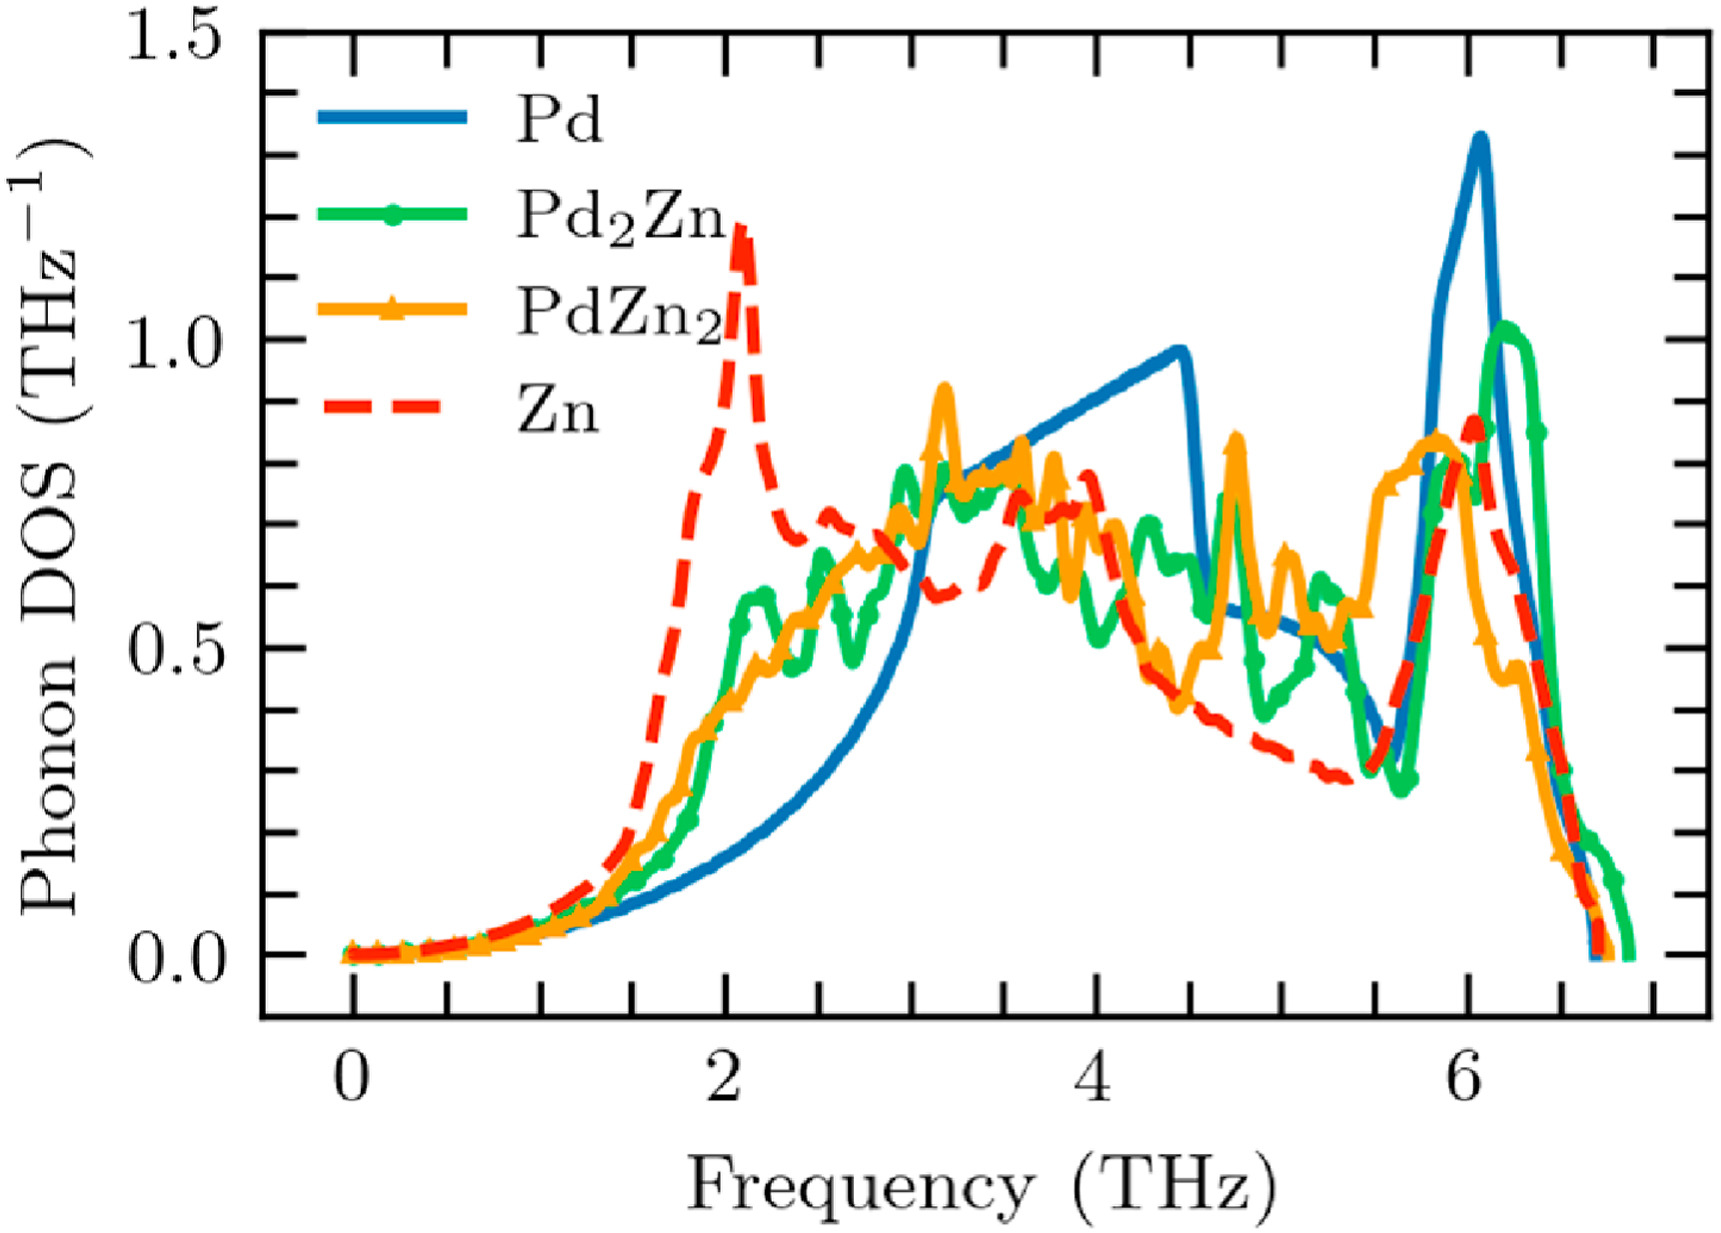
\includegraphics[width=0.5\textwidth]{intermetallics/Intermetallics-PdZnDOS.jpg}
    \caption{Predicted phonon DOS of Pd, Zn, Pd$_2$Zn and PdZn$_2$ from the DFT-based phonon calculations.}
    \label{intermetallics:fig:PdZnDOS}
\end{figure}

Figure \ref{intermetallics:fig:PdZnQHAPd} and Figure \ref{intermetallics:fig:PdZnQHAZn} show the comparison of the entropy and enthalpy of FCC-Pd and HCP-Zn from the phonon calculations to the SGTE pure element database \cite{dinsdale1991sgte}. Both show excellent agreement. For results of Pd obtained from phonon calculations and SGTE, the difference of enthalpy is less than 6.5\% and that of entropy is less than 5\%. The results of Zn show the difference of enthalpy less than 2.1\% and that of entropy less than 3.5\%.

\begin{figure}[H]
    \centering
    \normalsize
    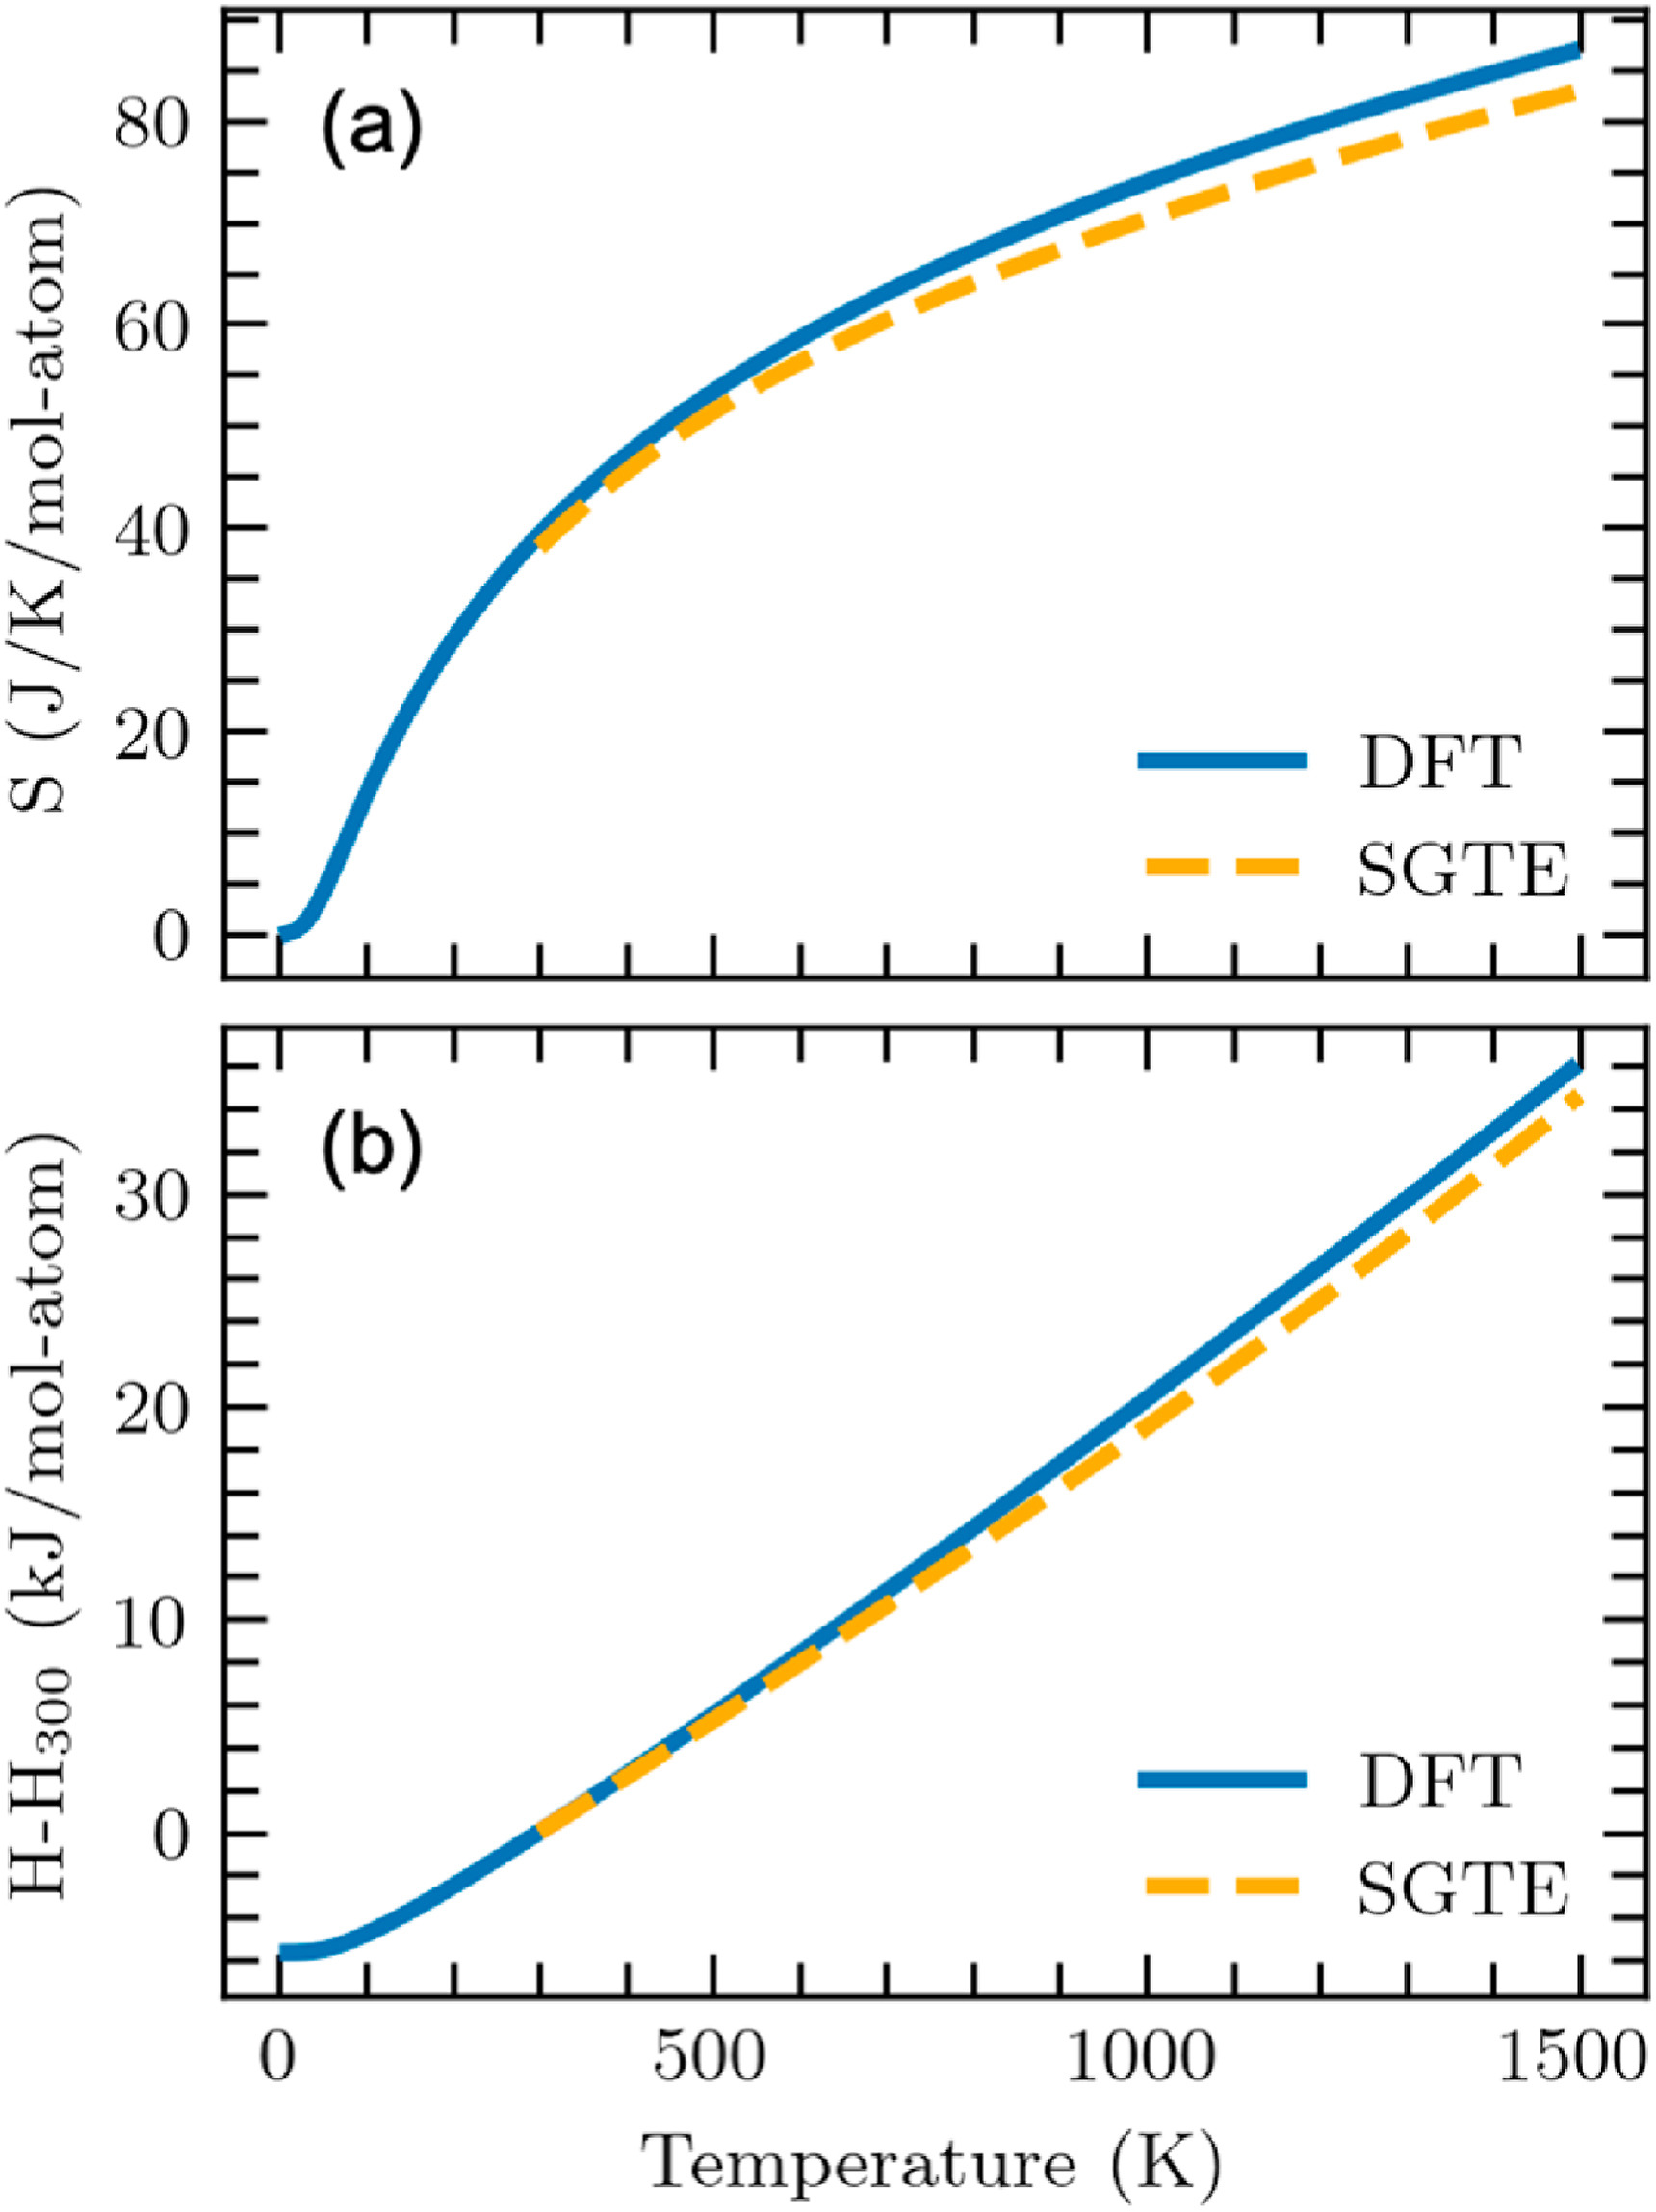
\includegraphics[width=0.4\textwidth]{intermetallics/Intermetallics-PdZnQHAPd.jpg}
    \caption{Comparison of the (a) entropy S and (b) enthalpy H $-$ H$_{300}$ of Pd from the DFT-based phonon calculations to the SGTE data \cite{dinsdale1991sgte}.}
    \label{intermetallics:fig:PdZnQHAPd}
\end{figure}

\begin{figure}[H]
    \centering
    \normalsize
    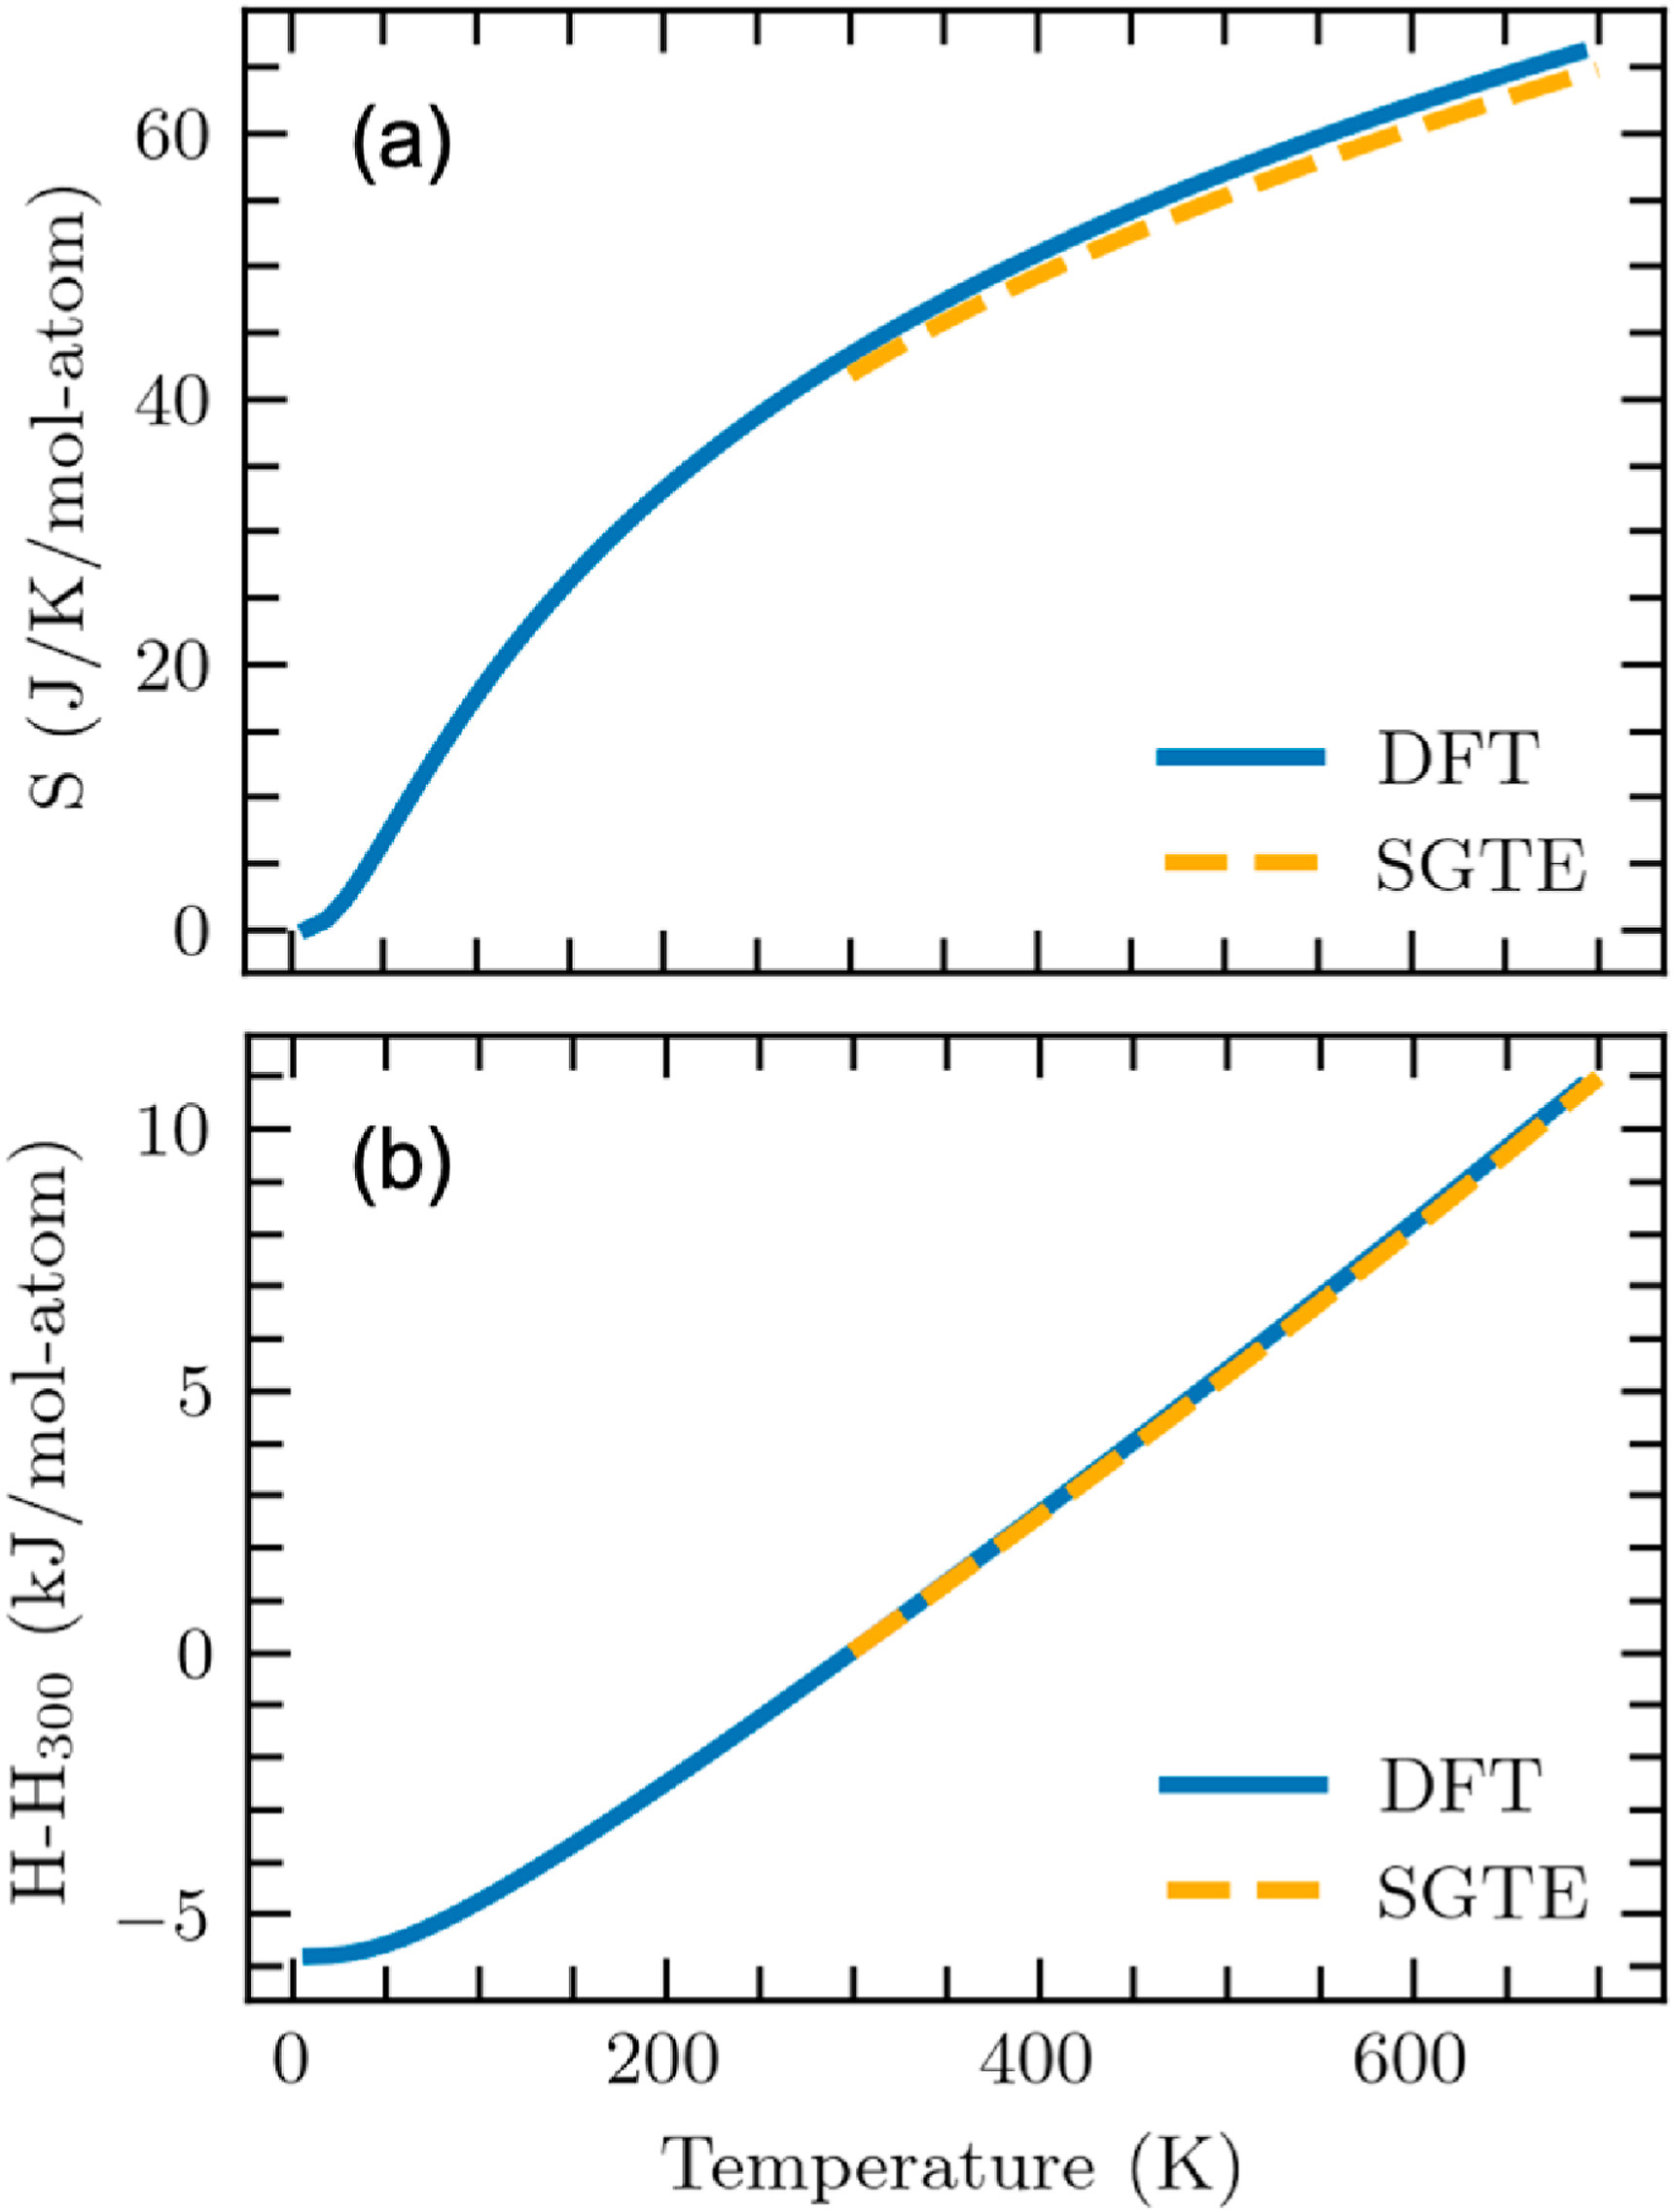
\includegraphics[width=0.4\textwidth]{intermetallics/Intermetallics-PdZnQHAZn.jpg}
    \caption{Comparison of the (a) entropy S and (b) enthalpy H $-$ H$_{300}$ of Zn from the DFT-based phonon calculations to the SGTE data \cite{dinsdale1991sgte}.}
    \label{intermetallics:fig:PdZnQHAZn}
\end{figure}

Table \ref{intermetallics:tab:PdZn_DFT_Hf} shows the enthalpy of formation $\Delta_f$H at 0 K predicted from the present DFT-based calculations using the exchange-correlation functionals of GGA and HSE06, along with experimental data \cite{ChiangIpserChang1977, kou1975thermodynamics}. For the $\gamma$ phase, the configuration of Pd$_{10}$Zn$_{42}$ ($x_{Zn}$ = 0.81) was used for DFT-based calculations and compared with experimental data at $x_{Zn}$ = 0.80. The $\Delta_f$H value predicted using HSE06 is $-33.7$ kJ/mol-atom, agreeing reasonably well with $-35.1$ kJ/mol-atom from experiments using calorimetry \cite{amore2009thermochemistry}. For the $\beta_1$ phase, the configuration of PdZn ($x_{Zn}$ = 0.50) was used. The $\Delta_f$H value of PdZn predicted using HSE06 is $-69.2$ kJ/mol-atom, which is in good agreement with measured $-73.9\pm10$ kJ/mol-atom reported by Chiang et al. \cite{ChiangIpserChang1977} and $-66.6$ kJ/mol-atom reported by Kou and Chang \cite{kou1975thermodynamics}, but is lower than the value predicted by GGA ($-53.7$ kJ/mol-atom). For both $\gamma$ and $\beta_1$ phases, the $\Delta_f$H values predicted by HSE06 are more accurate than those predicted by PBE-GGA. Considering the high computational cost, HSE06 was only applied for key endmembers close or on the convex hull in the present work such as (Zn)$_2$(Pd)$_3$(Pd)$_2$(Pd)$_6$ and (Zn)$_2$(Zn)$_3$(Pd)$_2$(Zn)$_6$. 

\begin{table}[H]
    \normalsize
    \centering
    \caption{Predicted enthalpy of formation at 0 K, $\Delta_f$H (kJ/mol-atom), of $\gamma$ and $\beta_1$ using DFT-based calculations with GGA and HSE06 as exchange-correlation functionals, respectively, in comparison with available experimental data.}
    \begin{tabular}{>{\raggedright\arraybackslash}m{2.5cm}>{\raggedright\arraybackslash}m{3cm}>{\raggedright\arraybackslash}m{2.5cm}>{\raggedright\arraybackslash}m{3cm}>{\raggedright\arraybackslash}m{3.5cm}}
    \hline
     \textbf{Phases} &  \textbf{Configurations} & \textbf{$x_{Zn}$} & \textbf{$\Delta_f$H} & \textbf{Source} \\
    \hline
    $\gamma$ phase & Pd$_{10}$Zn$_{42}$ & 0.81 & $-27.9$ & DFT/GGA\\
        & Pd$_{10}$Zn$_{42}$ & 0.81 & $-33.7$ & DFT/HSE06\\
       & N/A & 0.80 & $-35.1$ & Expt. at 300 K \cite{amore2009thermochemistry}\\
    $\beta_1$ phase & PdZn & 0.5 & $-53.7$ & DFT/GGA\\
       & PdZn & 0.5 & $-69.2$ & DFT/HSE06\\
       & PdZn & 0.5 & $-73.9\pm10$ & Expt. at 1273 K \cite{ChiangIpserChang1977}\\
       & PdZn & 0.5 & $-66.6$ & Expt. at 1273 K \cite{kou1975thermodynamics}\\
    \hline
    \end{tabular}
    \label{intermetallics:tab:PdZn_DFT_Hf}
\end{table}

\subsection{Thermodynamic modeling and phase equilibria} \label{intermetallics:ssec:PdZneq}
Figure \ref{Intermetallics:fig:PdZnPhaseDiagram} shows the calculated phase diagram in comparison with experimental data \cite{vizdal2006experimental, nowotny1951beitrag, alasafi1978mischung}, showing a good agreement, particularly the phase boundaries of the $\gamma$ phase. The max difference between calculated and experimental Zn compositions of the $\gamma$ phase  $x_{Zn}^{Cal}-x_{Zn}^{Expt.}$ is around 0.016 at 892 K. The solubility range of the $\gamma$ phase is between $x_{Zn} = 0.775 - 0.846$ from 300 K to 1000 K. The congruent melting temperature of the $\gamma$ phase is 1150 K in good agreement with 1153 K suggested by Massalski \cite{massalski1986binary}.\\

\begin{figure}[H]
    \centering
    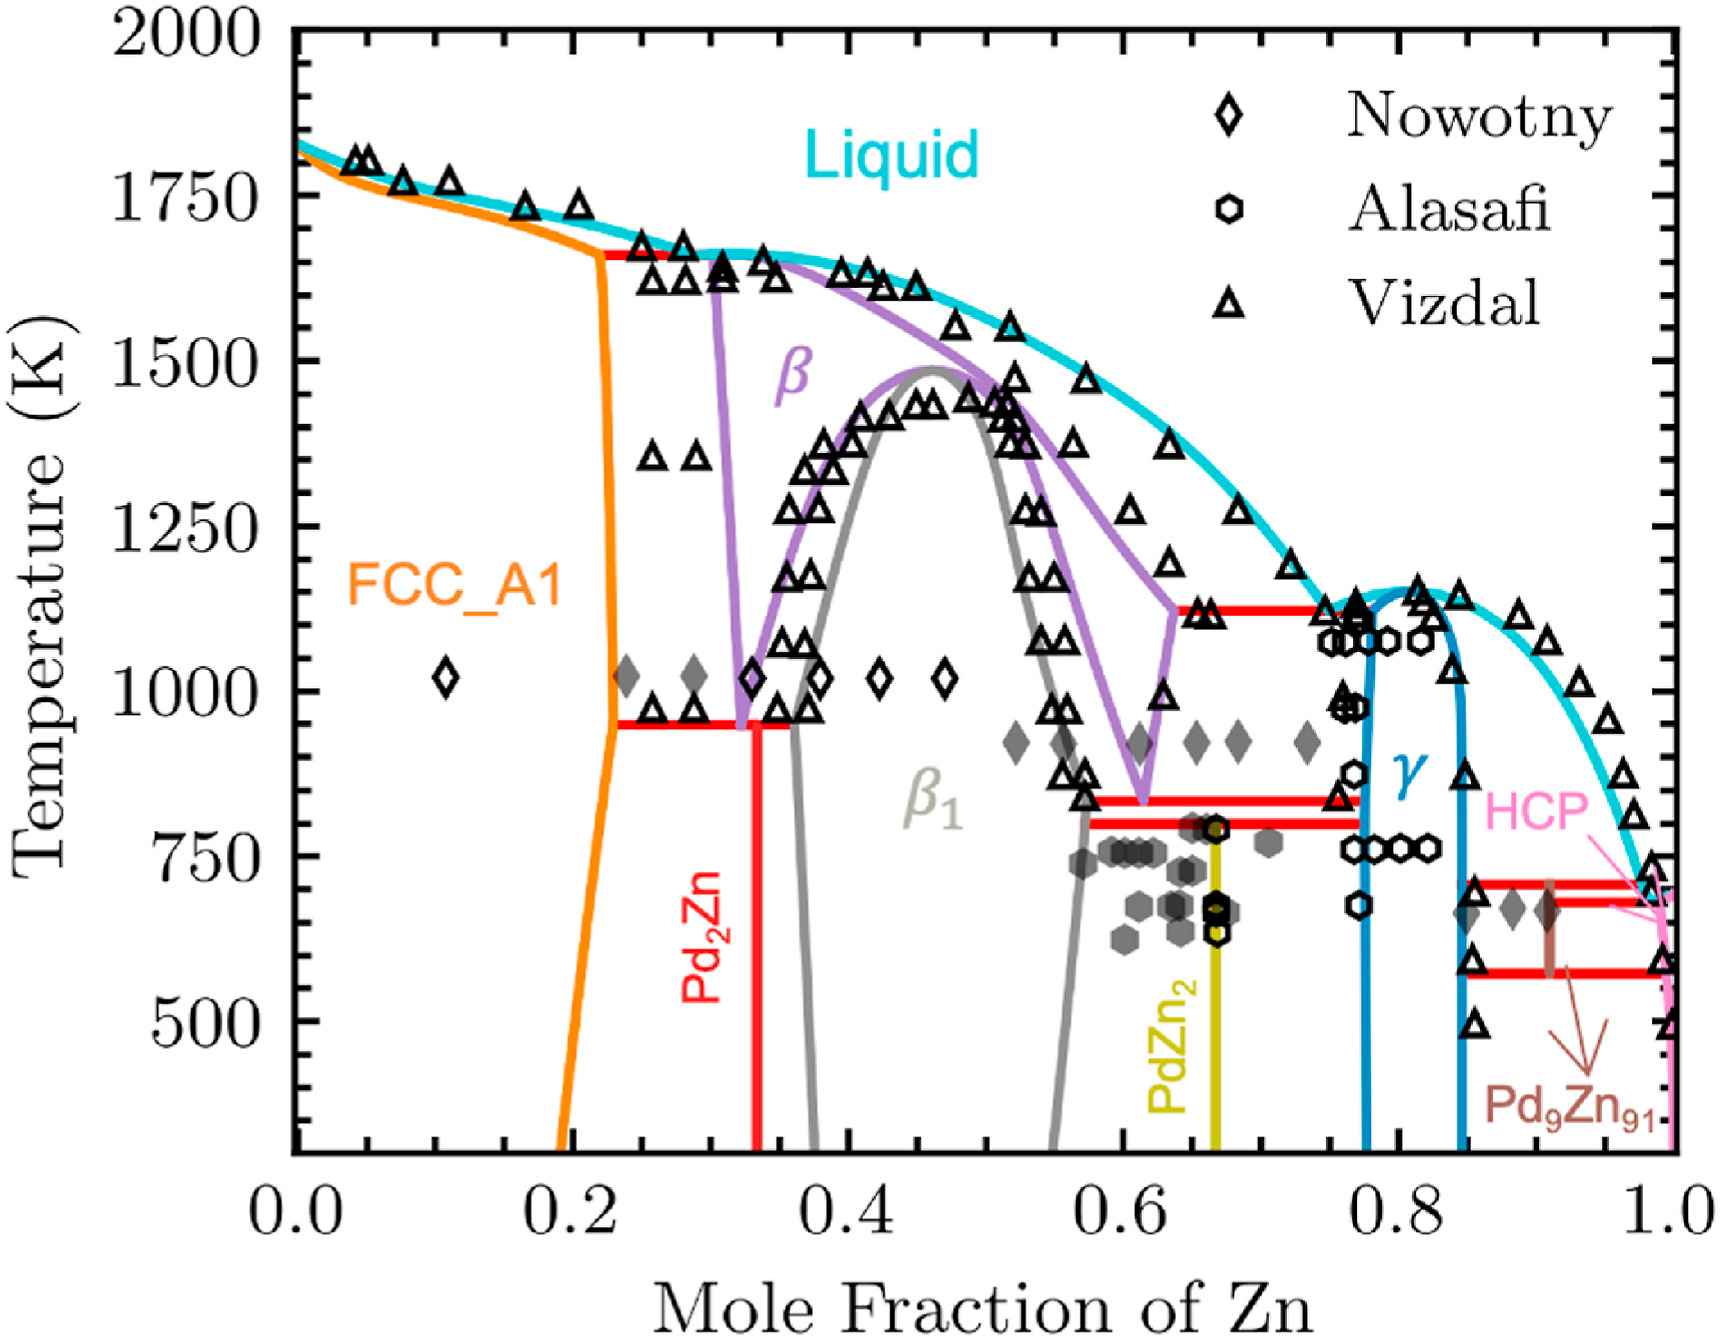
\includegraphics[width=0.6\linewidth]{intermetallics/Intermetallics-PdZnPhaseDiagram.jpg}
    \caption{Calculated phase diagram from the present CALPHAD modeling in comparison with experimental data from Nowotny et al. \cite{nowotny1951beitrag} (diamonds), Alasafi et al. \cite{alasafi1978mischung} (hexagons), and experimental data summarized by Vizdal et al. \cite{vizdal2006experimental} (triangles). Hollow diamonds and hexagons represent single phase region and shadowed diamonds and hexagons represent two phase regions reported by Nowotny et al. \cite{nowotny1951beitrag} and Alasafi et al. \cite{alasafi1978mischung}.}
    \label{Intermetallics:fig:PdZnPhaseDiagram}
\end{figure} 

Table \ref{intermetallics:tab:inv} lists the temperatures and compositions of invariant reactions. The experimentally reported invariant reactions, i.e., Liquid $\rightarrow$ Pd$_9$Zn$_{91}$ $+$ HCP by Vizdal et al. \cite{vizdal2006experimental} and other four invariant reactions by Massalski \cite{massalski1986binary}, are well reproduced. The largest discrepancy is seen for the eutectic reaction, Liquid $\rightarrow$ Pd$_9$Zn$_{91}$ + HCP, i.e., 681 K calculated from the present work versus 690 K in the literature \cite{vizdal2006experimental}.

\begin{table}[H]
    \centering
    \caption{Temperatures and compositions of invariant reactions in the Pd-Zn system calculated from the present CALPHAD modeling with available experimental data included.}
    \begin{tabular}{>{\raggedright\arraybackslash}m{5cm}>{\raggedright\arraybackslash}m{1cm}>{\raggedright\arraybackslash}m{1cm}>{\raggedright\arraybackslash}m{1cm}>{\raggedright\arraybackslash}m{3cm}>{\raggedright\arraybackslash}m{2.5cm}}
        \hline
         \textbf{Reaction}& \textbf{$x_{Zn}$} & (\%) &  & \textbf{Temperature (K)} & \textbf{Ref.}\\
        \hline
        Liquid $\rightarrow \beta + \gamma$&74.9&63.7&78.1&1122.1&This work\\
         &75&65&77&1118&Expt.\cite{massalski1986binary}\\
         $\beta \rightarrow \beta_1 + \gamma$&61.5&57.3&77.5&834&This work\\
	&57&55&76&838&Expt.\cite{massalski1986binary}\\
        $\beta_1 + \gamma \rightarrow$ PdZn$_2$&57.2&77.5&66.7&799.6&This work\\
	&56&76&66.7&$803\pm10$&Expt.\cite{massalski1986binary}\\
        Liquid $+ \gamma \rightarrow$ Pd$_9$Zn$_{91}$&97.7&84.6&91.0&707.2&This work\\
	&98&85&92&703&Expt.\cite{hansen1958constitution}\\
	&&&&707&Expt.\cite{vizdal2006experimental}\\
        Liquid $\rightarrow$ Pd$_9$Zn$_{91}$ $+$ HCP&98.2&91.0&99.0&681.1&This work\\
	&&&&690&Expt.\cite{vizdal2006experimental}\\
         \hline
    \end{tabular}
    \label{intermetallics:tab:inv}
\end{table}

Figure \ref{intermetallics:fig:PdZnQHAPd2Zn} and Figure \ref{intermetallics:fig:PdZnQHAPdZn2} show the heat capacity, entropy, and enthalpy of stoichiometric compounds Pd$_2$Zn and PdZn$_2$ from the present model in comparison with results from the phonon calculations. Good agreement is found, especially for enthalpy with a difference less than 4.7\% for Pd$_2$Zn and 2.8\% for PdZn$_2$. The entropy of PdZn$_2$ from phonon calculations compared with the present model shows the largest discrepancy with a difference of around 6.5 J/mol-atom-K. This is because the model parameters of stoichiometric compounds, which are obtained from first-principles calculated enthalpy and entropy, were adjusted with the experimental data of the peritectoid temperature.

\begin{figure}[H]
    \centering
    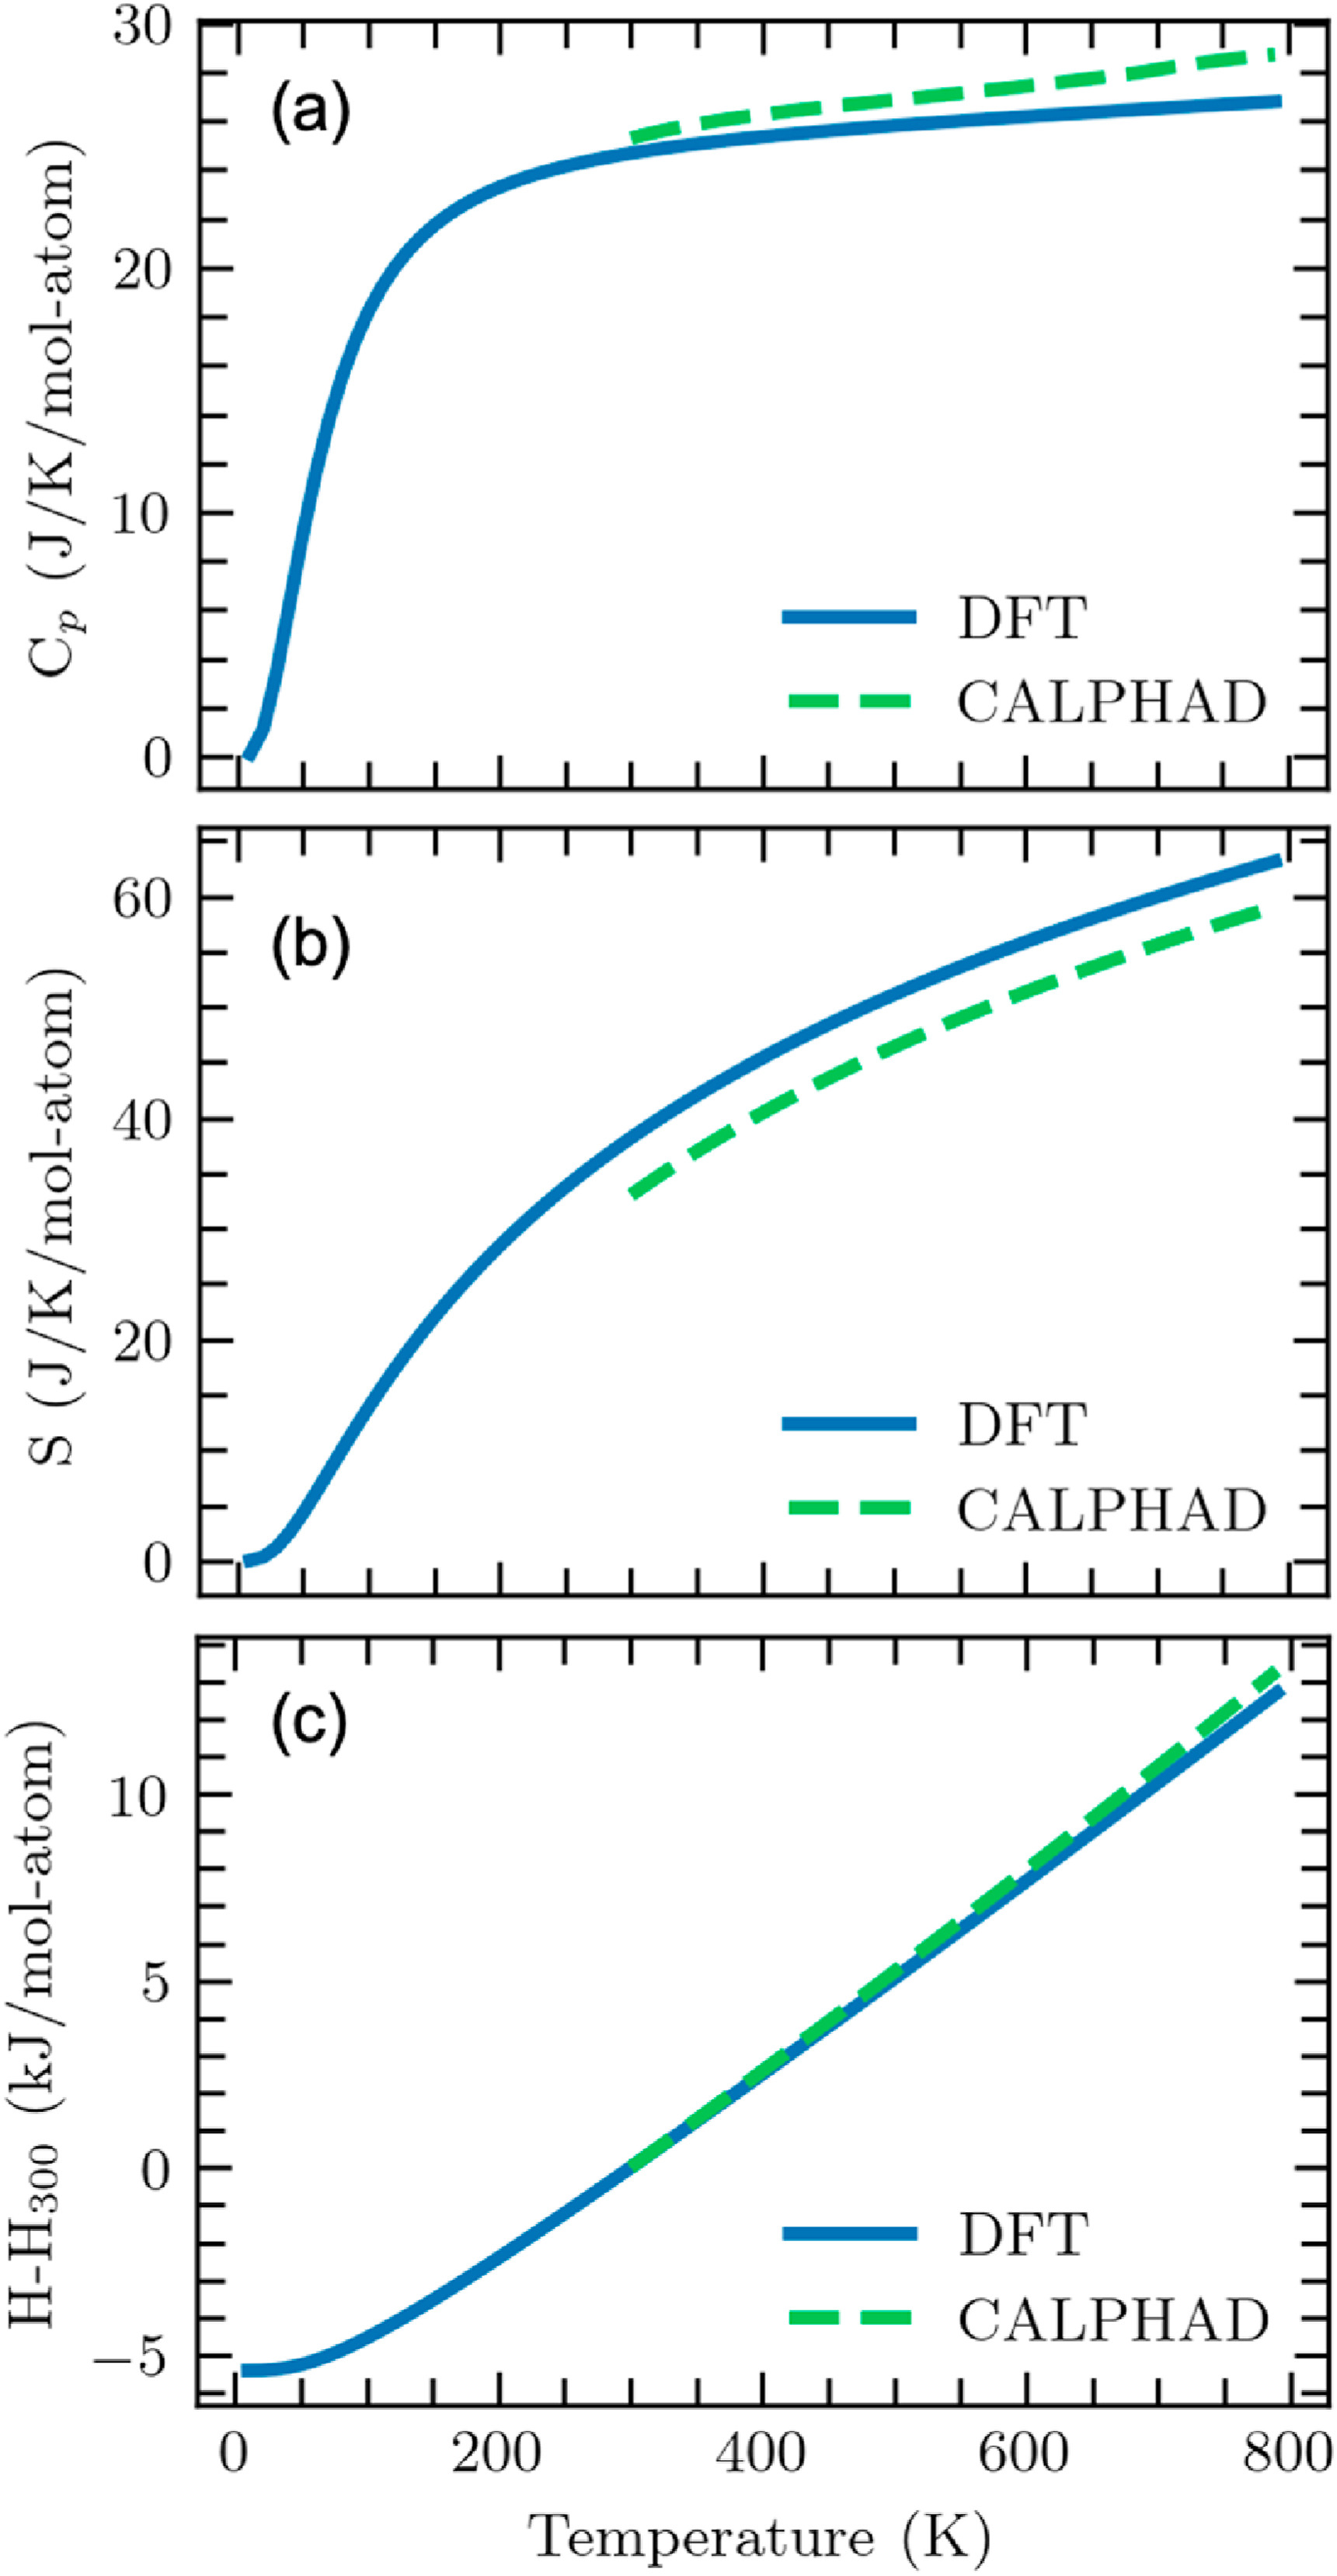
\includegraphics[width=0.5\linewidth]{intermetallics/Intermetallics-PdZnQHAPd2Zn.jpg}
    \caption{Predicted (a) heat capacity C$_p$, (b) entropy S, and (c) enthalpy H $-$ H$_{300}$ of Pd$_2$Zn using the present results form DFT-based phonon calculations, compared with those from the present CALPHAD modeling.}
    \label{intermetallics:fig:PdZnQHAPd2Zn}
\end{figure}

\begin{figure}[H]
    \centering
    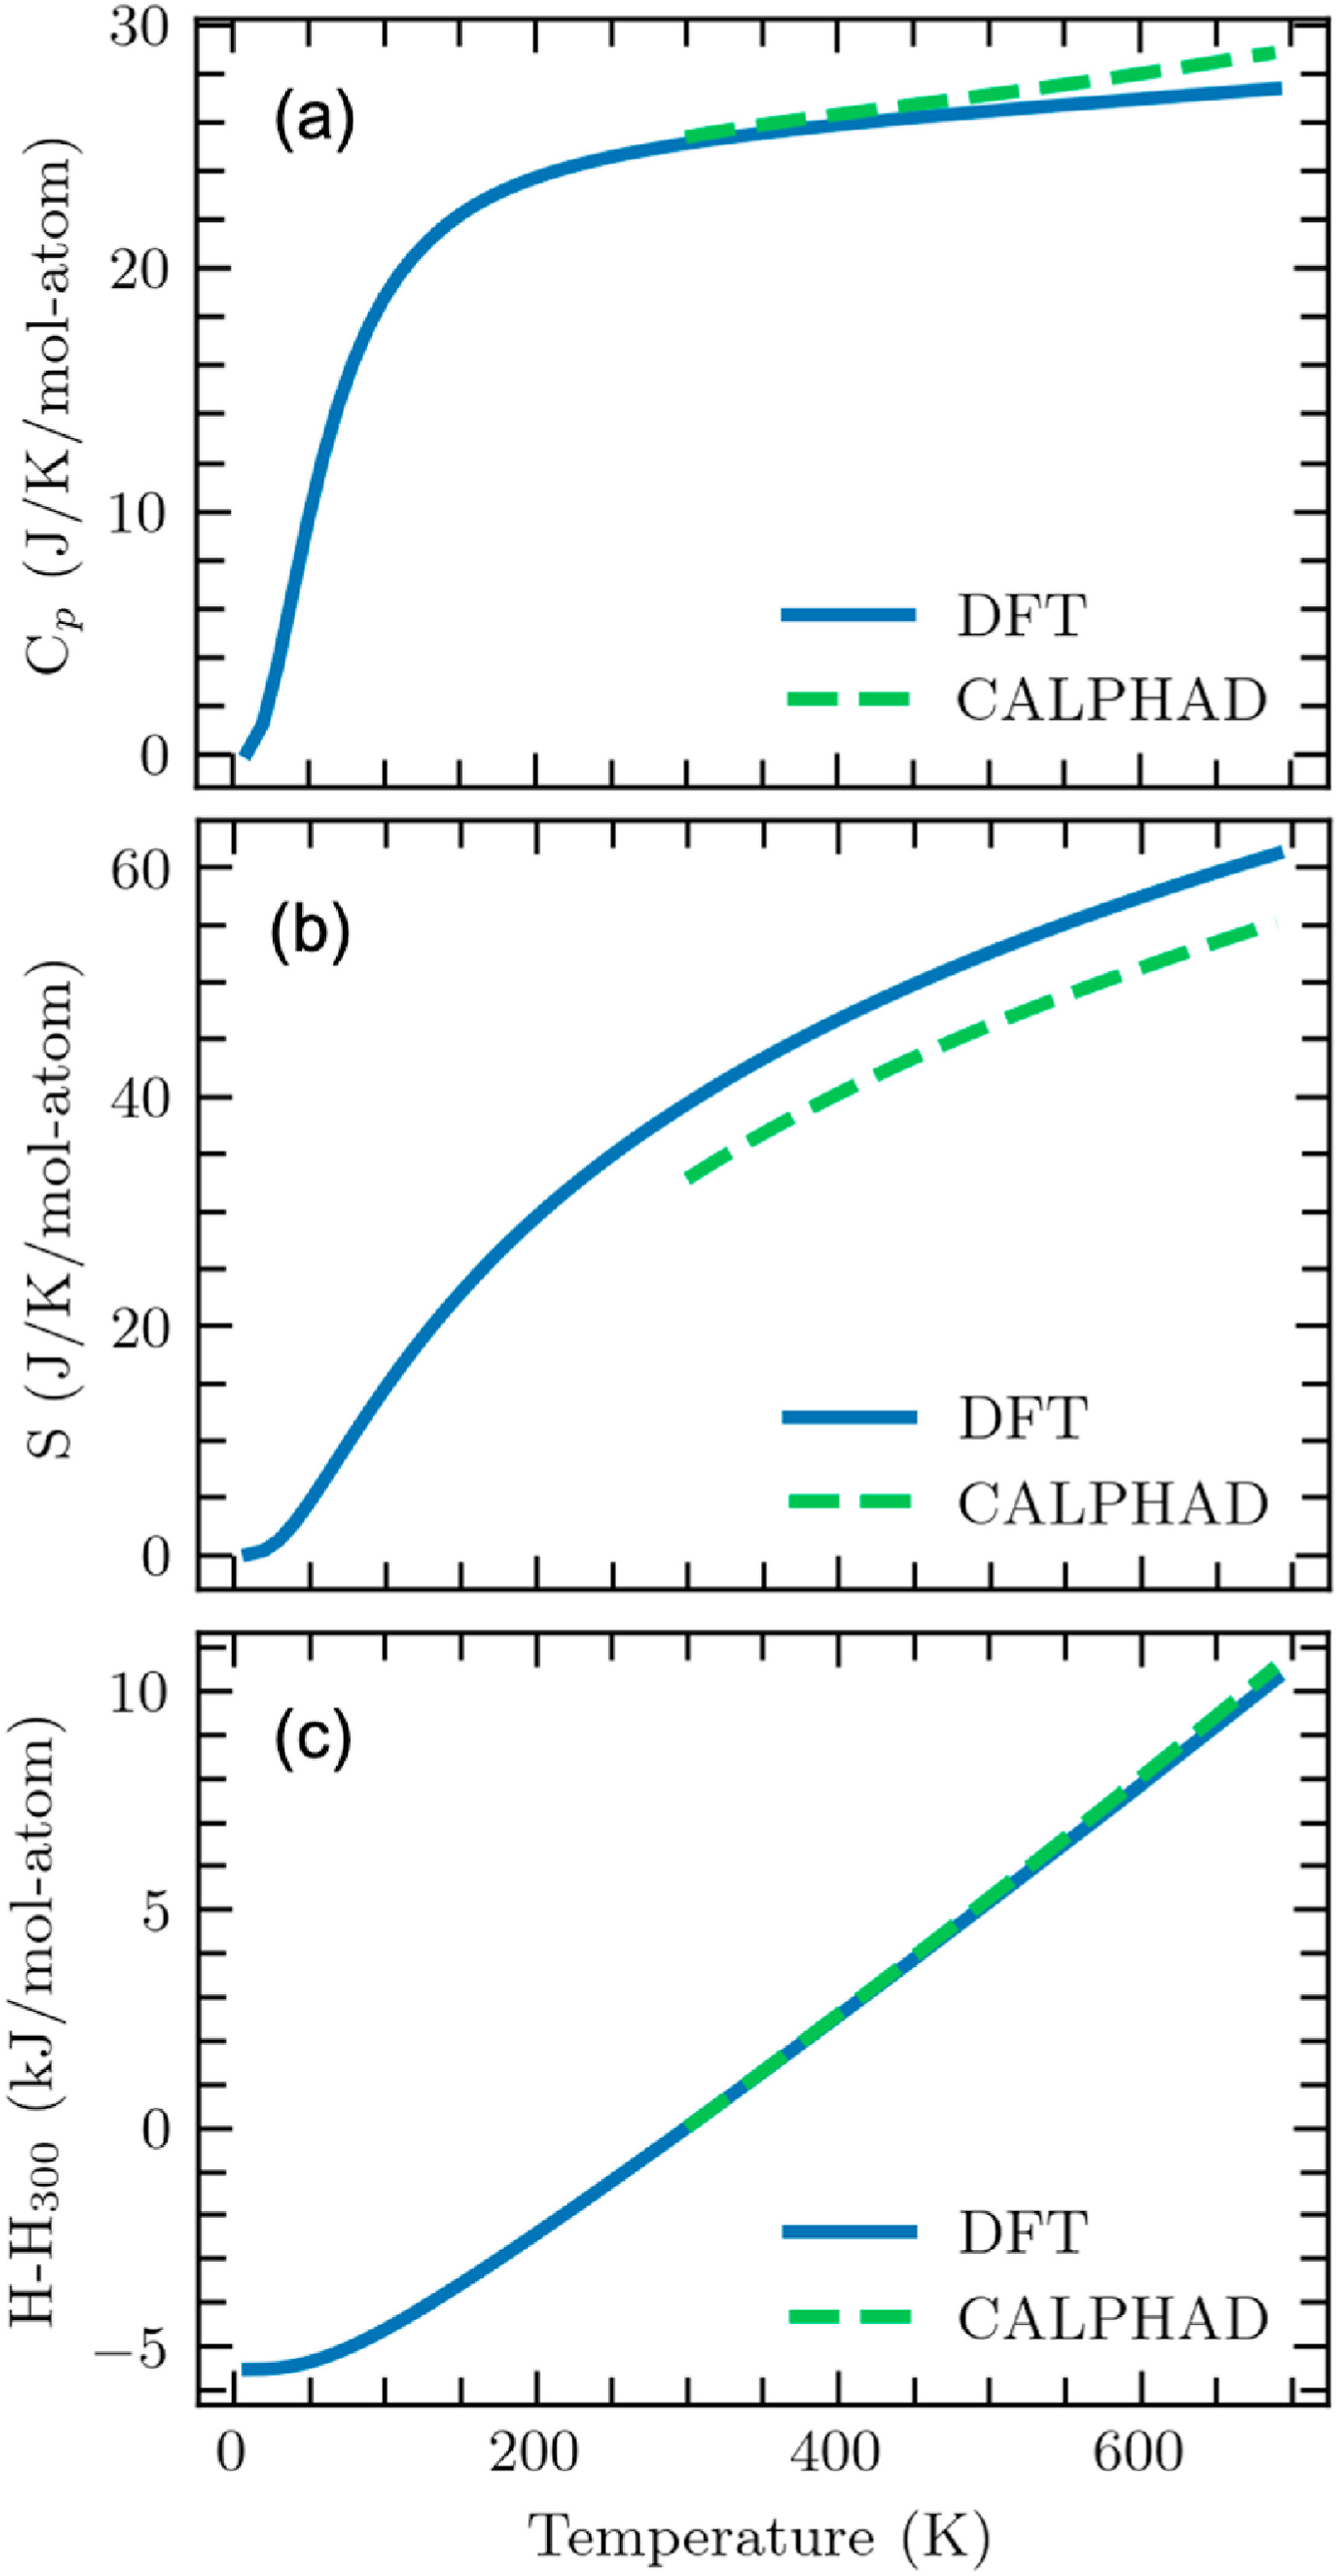
\includegraphics[width=0.5\linewidth]{intermetallics/Intermetallics-PdZnQHAPdZn2.jpg}
    \caption{Predicted (a) heat capacity C$_p$, (b) entropy S, and (c) enthalpy H $-$ H$_{300}$ of PdZn$_2$ using the present results form DFT-based phonon calculations, compared with those from the present CALPHAD modeling.}
    \label{intermetallics:fig:PdZnQHAPdZn2}
\end{figure}

The parameters of the FCC\_A1 phase in the database were optimized based on phase boundary data and activity data of the FCC\_A1 phase. Considering fitting different types of data, a balanced modeling result between phase boundary data and activity data is chosen. The experimental data for liquidus and solidus on the Pd-rich side are scarce. In the present work, data for liquidus and solidus in the Pd-rich side summarized by Vizdal et al. \cite{vizdal2006experimental} are used for modeling, thus the shape of liquidus and solidus in the Pd-rich side followed the trend of experimental data. Figure \ref{intermetallics:fig:PdZnACR} shows the activity values of Zn at 1273 K calculated from the present model in comparison with experimental data by Chiang et al. \cite{ChiangIpserChang1977}. The activity values of Zn in $\beta_1$ from the present model agree well with the experiments \cite{ChiangIpserChang1977} with the mean absolute error of $\ln{a_{Zn}}$ being 0.4. A higher discrepancy occurs in the composition range $x_{Zn}$ = 0.51-0.6. For example, at $x_{Zn}$ = 0.55, $\ln{a_{Zn}}$ calculated from the present model is $-3.52$ compared with -1.56 measured by Chiang et al. \cite{ChiangIpserChang1977}. They reported a single $\beta_1$ phase for $x_{Zn}$ = 0.52 and a single $\beta$ phase for $x_{Zn}$ = 0.6. However, the present work predicts that $\beta_1$ is in equilibrium with $\beta$ at $x_{Zn}$ = 0.52, and $\beta$ is in equilibrium with Liquid at $x_{Zn}$=0.6 (see Figure \ref{Intermetallics:fig:PdZnPhaseDiagram}). Figure \ref{intermetallics:fig:PdZnACRUQ} shows the activity values of Zn in FCC, $\beta$, and $\beta_1$ phases, respectively, calculated from the present model with the shaded regions for the uncertainty of each phase. For FCC, larger uncertainty occurs when $x_{Zn}$ < 0.2, where the largest uncertainty is around $\pm15$\% from the mean value at $x_{Zn}$ = 0.02, and experimental data are located within this uncertainty region. For $\beta_1$, the experimental data are in the uncertainty region when $x_{Zn}$ < 0.5, and the largest error is around $x_{Zn}$ = 0.52 with $\ln{a_{Zn}}$ = $-1.66$ from experiments \cite{ChiangIpserChang1977} compared with $-3.35$ calculated from the present model. For $\beta$, $\ln{a_{Zn}} = -10.33$ from experiments \cite{ChiangIpserChang1977} at $x_{Zn}$ = 0.3 are closer to the lower limit of the uncertainty region, where $\ln{a_{Zn}}$ at the lower uncertainty is $-10.81$. The shaded ranges in Figure \ref{intermetallics:fig:PdZnACRUQ} decrease with increasing $x_{Zn}$, indicating a larger uncertainty of activity occurs in the Pd-rich region. 

\begin{figure}[H]
    \centering
    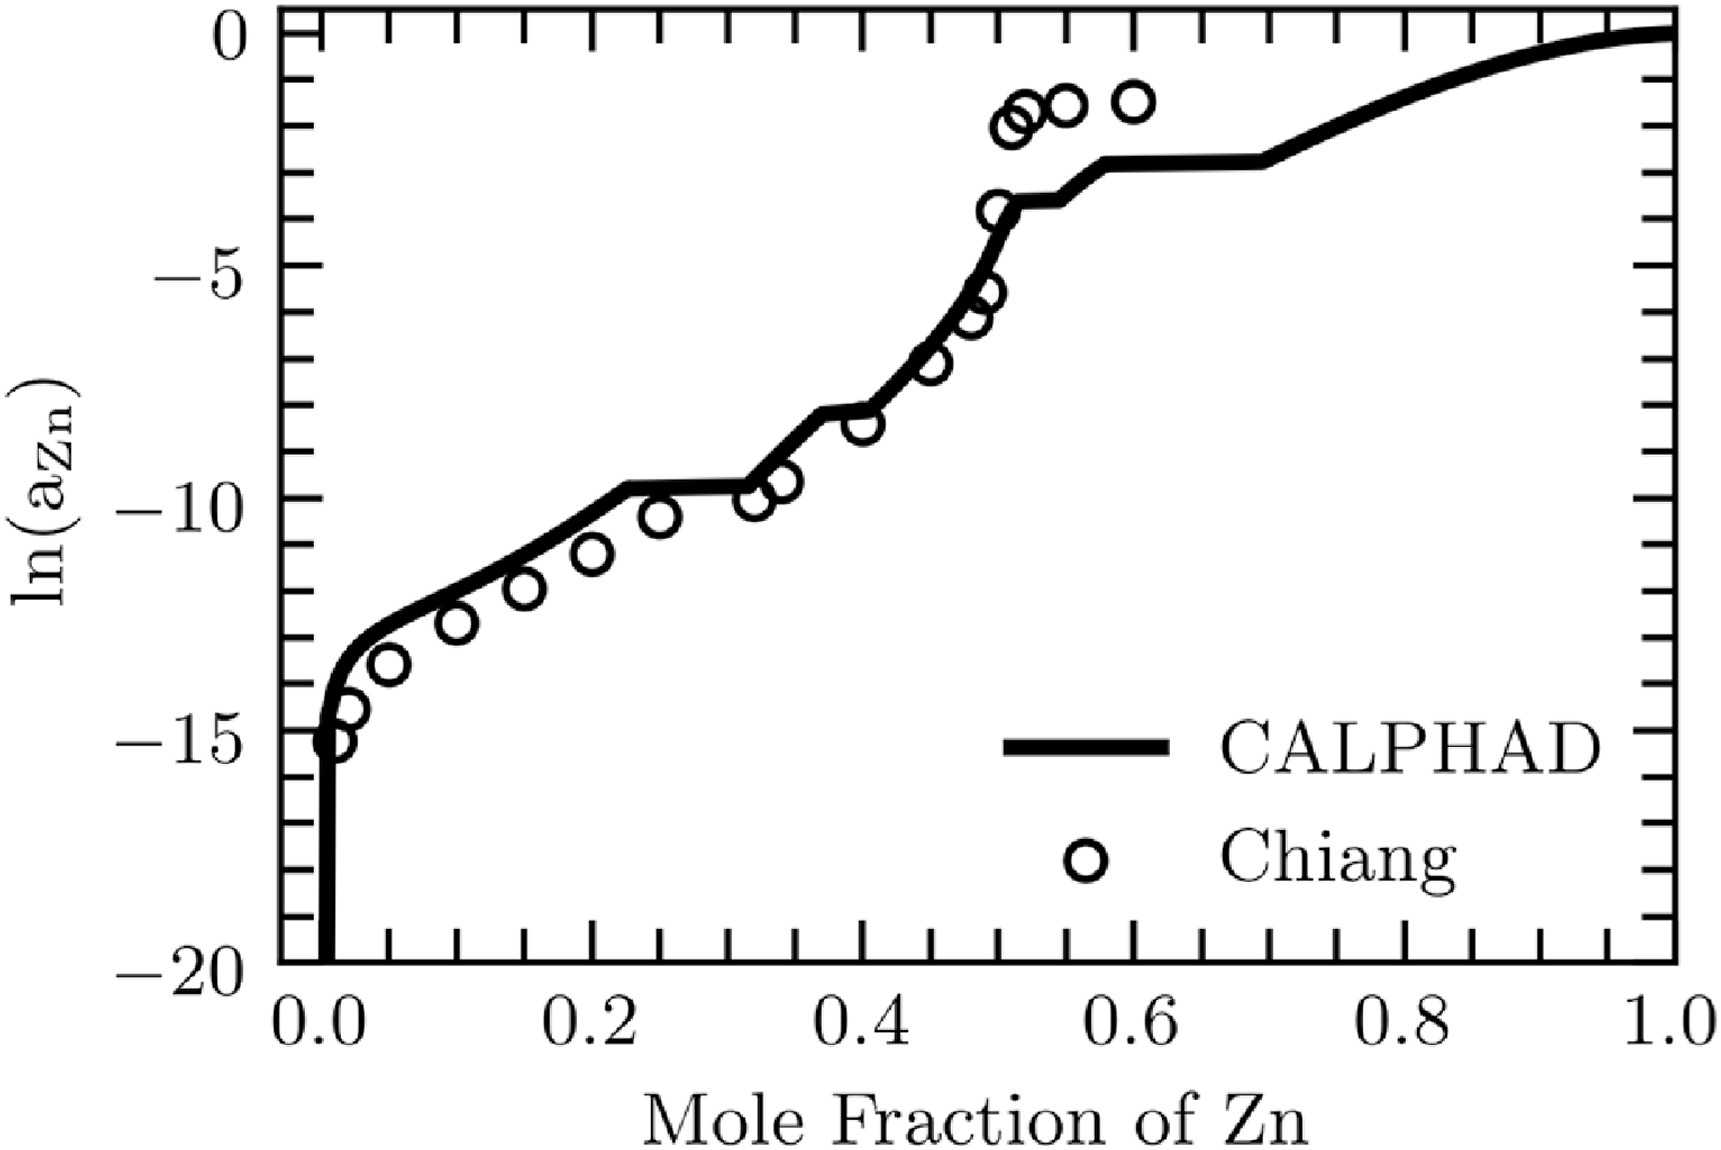
\includegraphics[width=0.5\linewidth]{intermetallics/Intermetallics-PdZnACR.jpg}
    \caption{Calculated activity of Zn at 1273 K with experimental data measured by Chiang et al. \cite{ChiangIpserChang1977} superimposed.}
    \label{intermetallics:fig:PdZnACR}
\end{figure}

\begin{figure}[H]
    \centering
    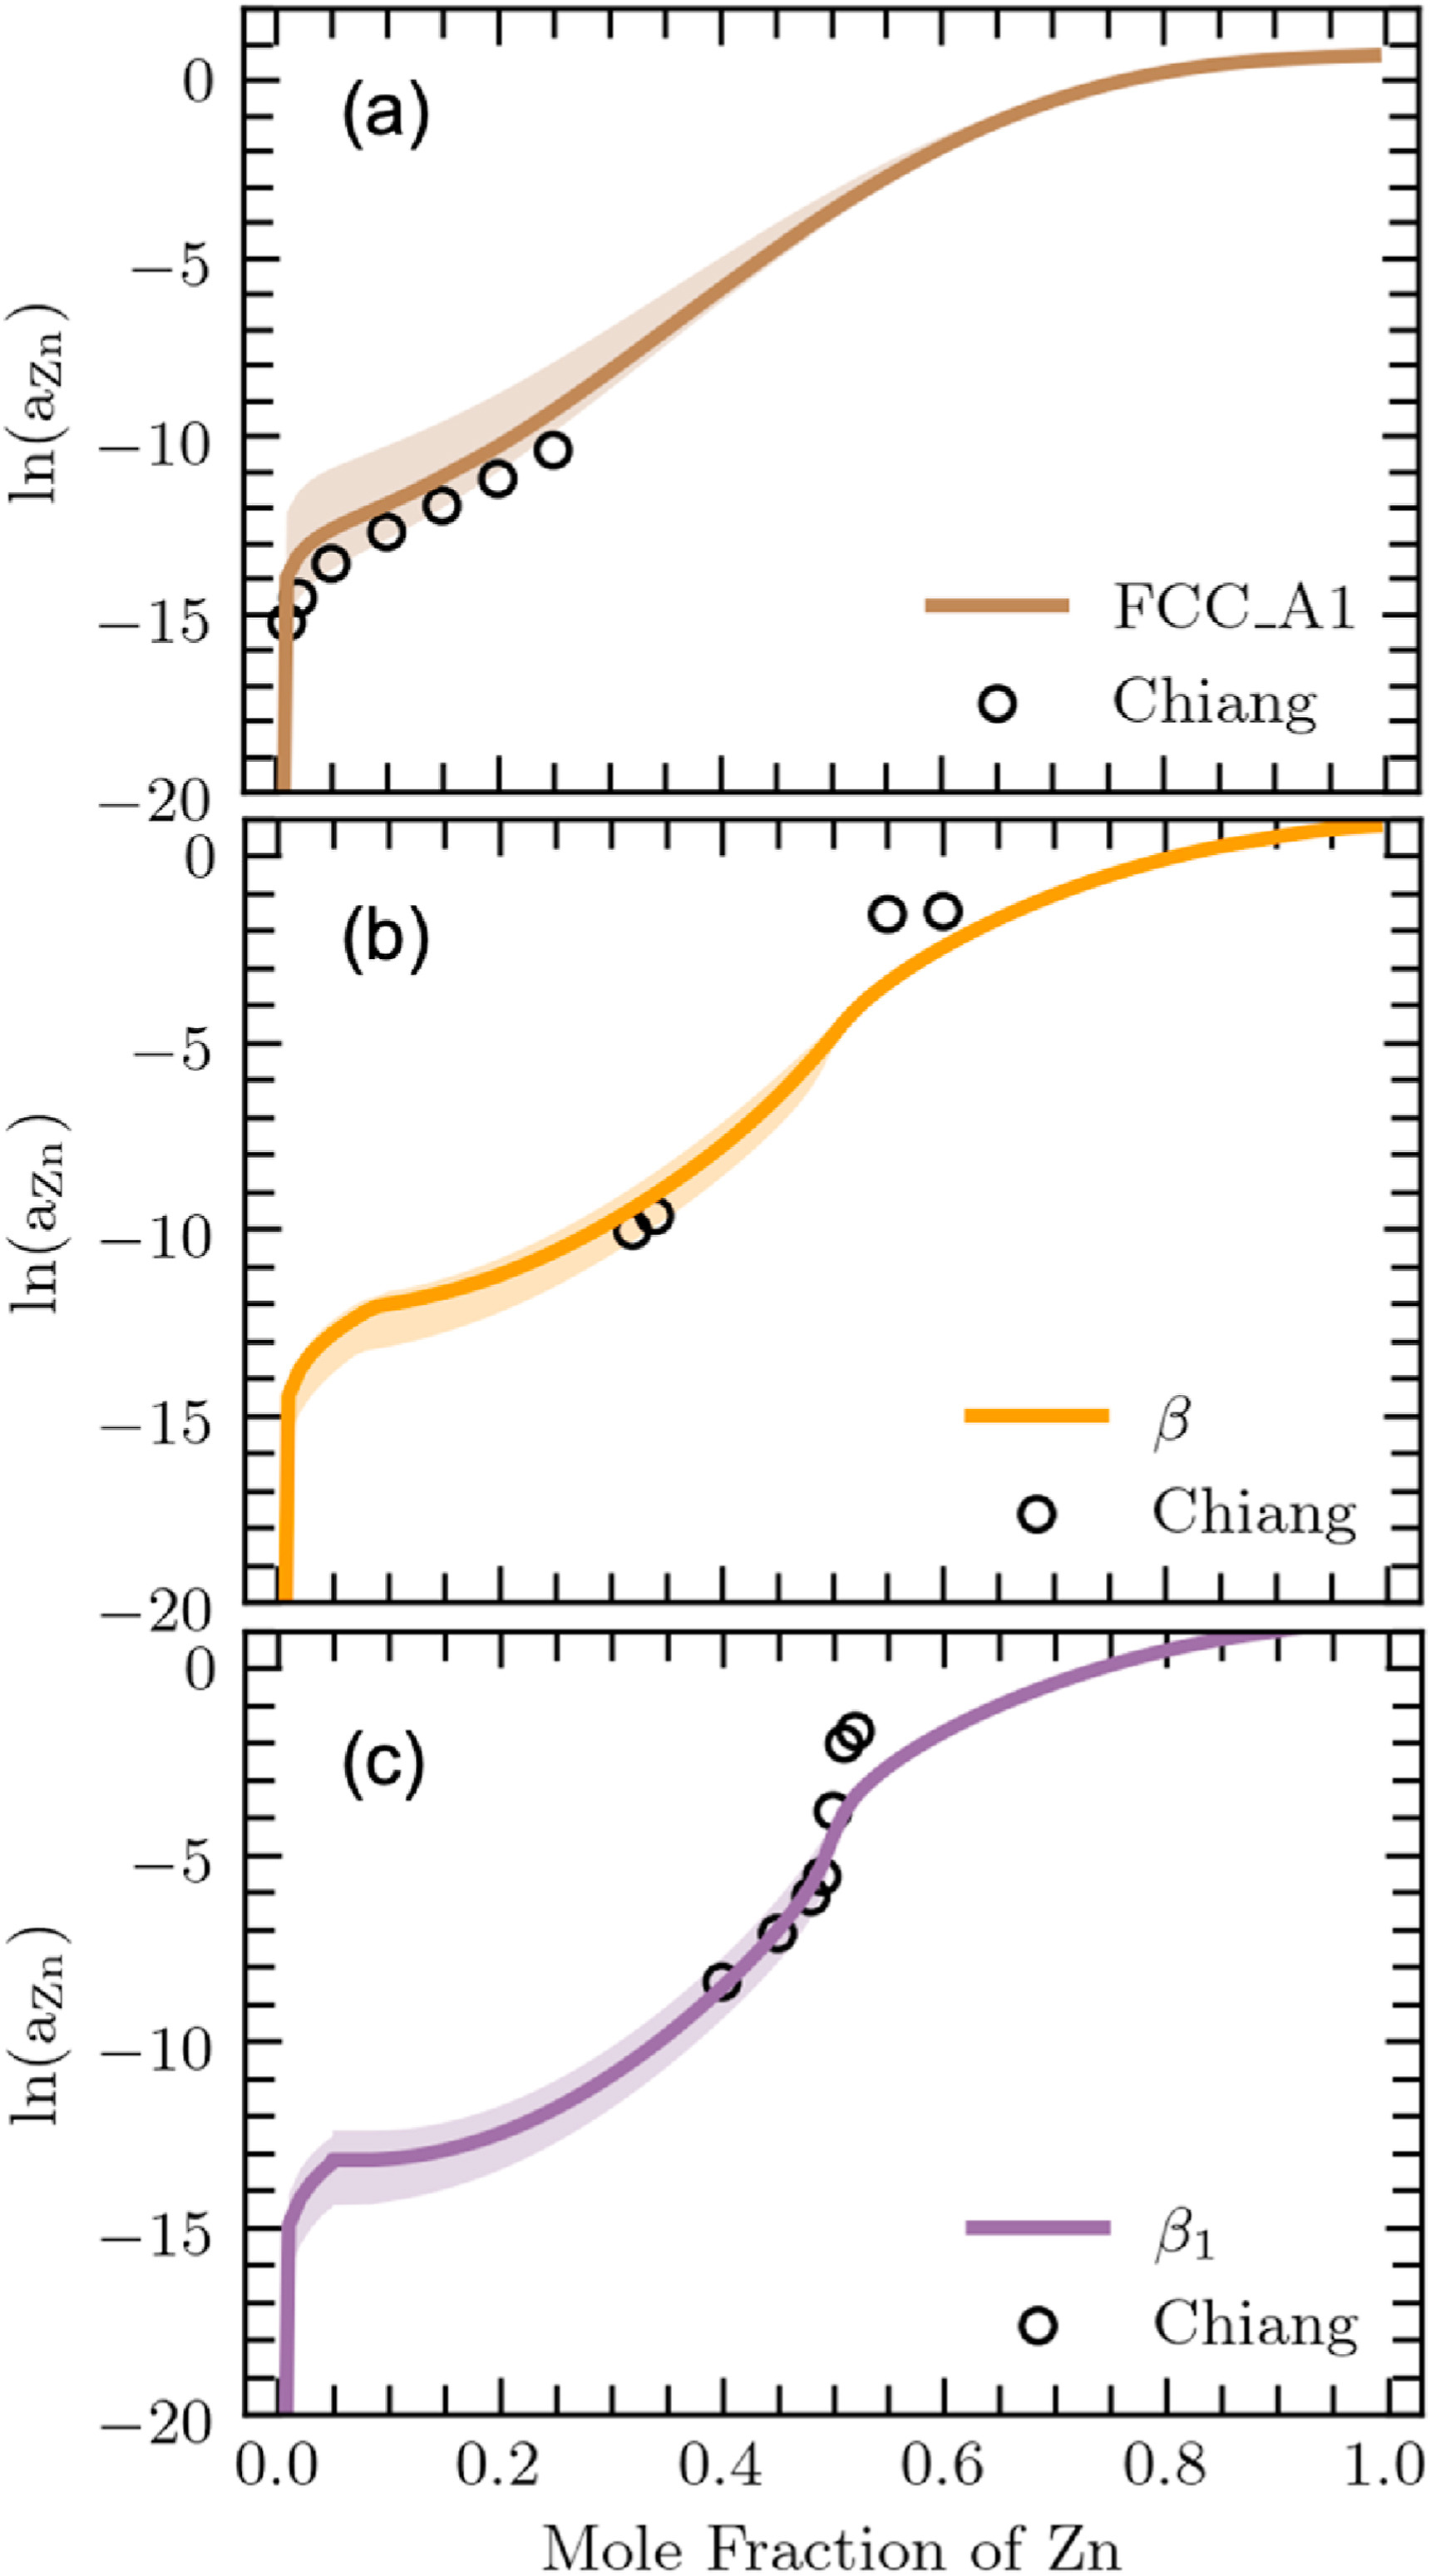
\includegraphics[width=0.5\linewidth]{intermetallics/Intermetallics-PdZnACRUQ.jpg}
    \caption{Uncertainty quantification of the activity of (a) FCC, (c) $\beta$, and (d) $\beta_1$, marked in the shaded regions with the corresponding color of each phase and compared with experimental data by Chiang et al. \cite{ChiangIpserChang1977}.}
    \label{intermetallics:fig:PdZnACRUQ}
\end{figure}

Figure \ref{intermetallics:fig:PdZnHMR} plots the enthalpy of formation $\Delta_f$H of the Pd-Zn phases at 1273 K and 300 K from the present model and available experimental data \cite{amore2009thermochemistry, ChiangIpserChang1977, kou1975thermodynamics}, along with the calculated results from the previous CALPHAD modeling \cite{vizdal2006experimental} at 300 K and the present first-principles results of the $\gamma$ phase at 0 K and high temperatures. $\Delta_f$H at 1273 K agrees reasonably well with experimental data \cite{ChiangIpserChang1977, kou1975thermodynamics}. $\Delta_f$H of $\beta_1$ at $x_{Zn}$ = 0.5 and 1273 K is $-70.1$ kJ/mol-atom from the present work, compared with -$73.9\pm10$ kJ/mol-atom measured by Chiang et al. \cite{ChiangIpserChang1977} and $-66.6$ kJ/mol-atom measured by Kou et al. \cite{kou1975thermodynamics}. Figure \ref{intermetallics:fig:PdZnHMR} shows that $\Delta_f$H of $\gamma$ from the present model has better agreement with experiments than the previous model \cite{vizdal2006experimental}. At $x_{Zn}$ = 0.8, $\Delta_f$H value of $\gamma$ from the present model is $-40.6$ kJ/mol-atom at 300 K and from the previous model \cite{vizdal2006experimental} is $-48.5$ kJ/mol-atom, compared with $-35.1$ kJ/mol-atom measured by Amore et al. \cite{amore2009thermochemistry}.

\begin{figure}[H]
    \centering
    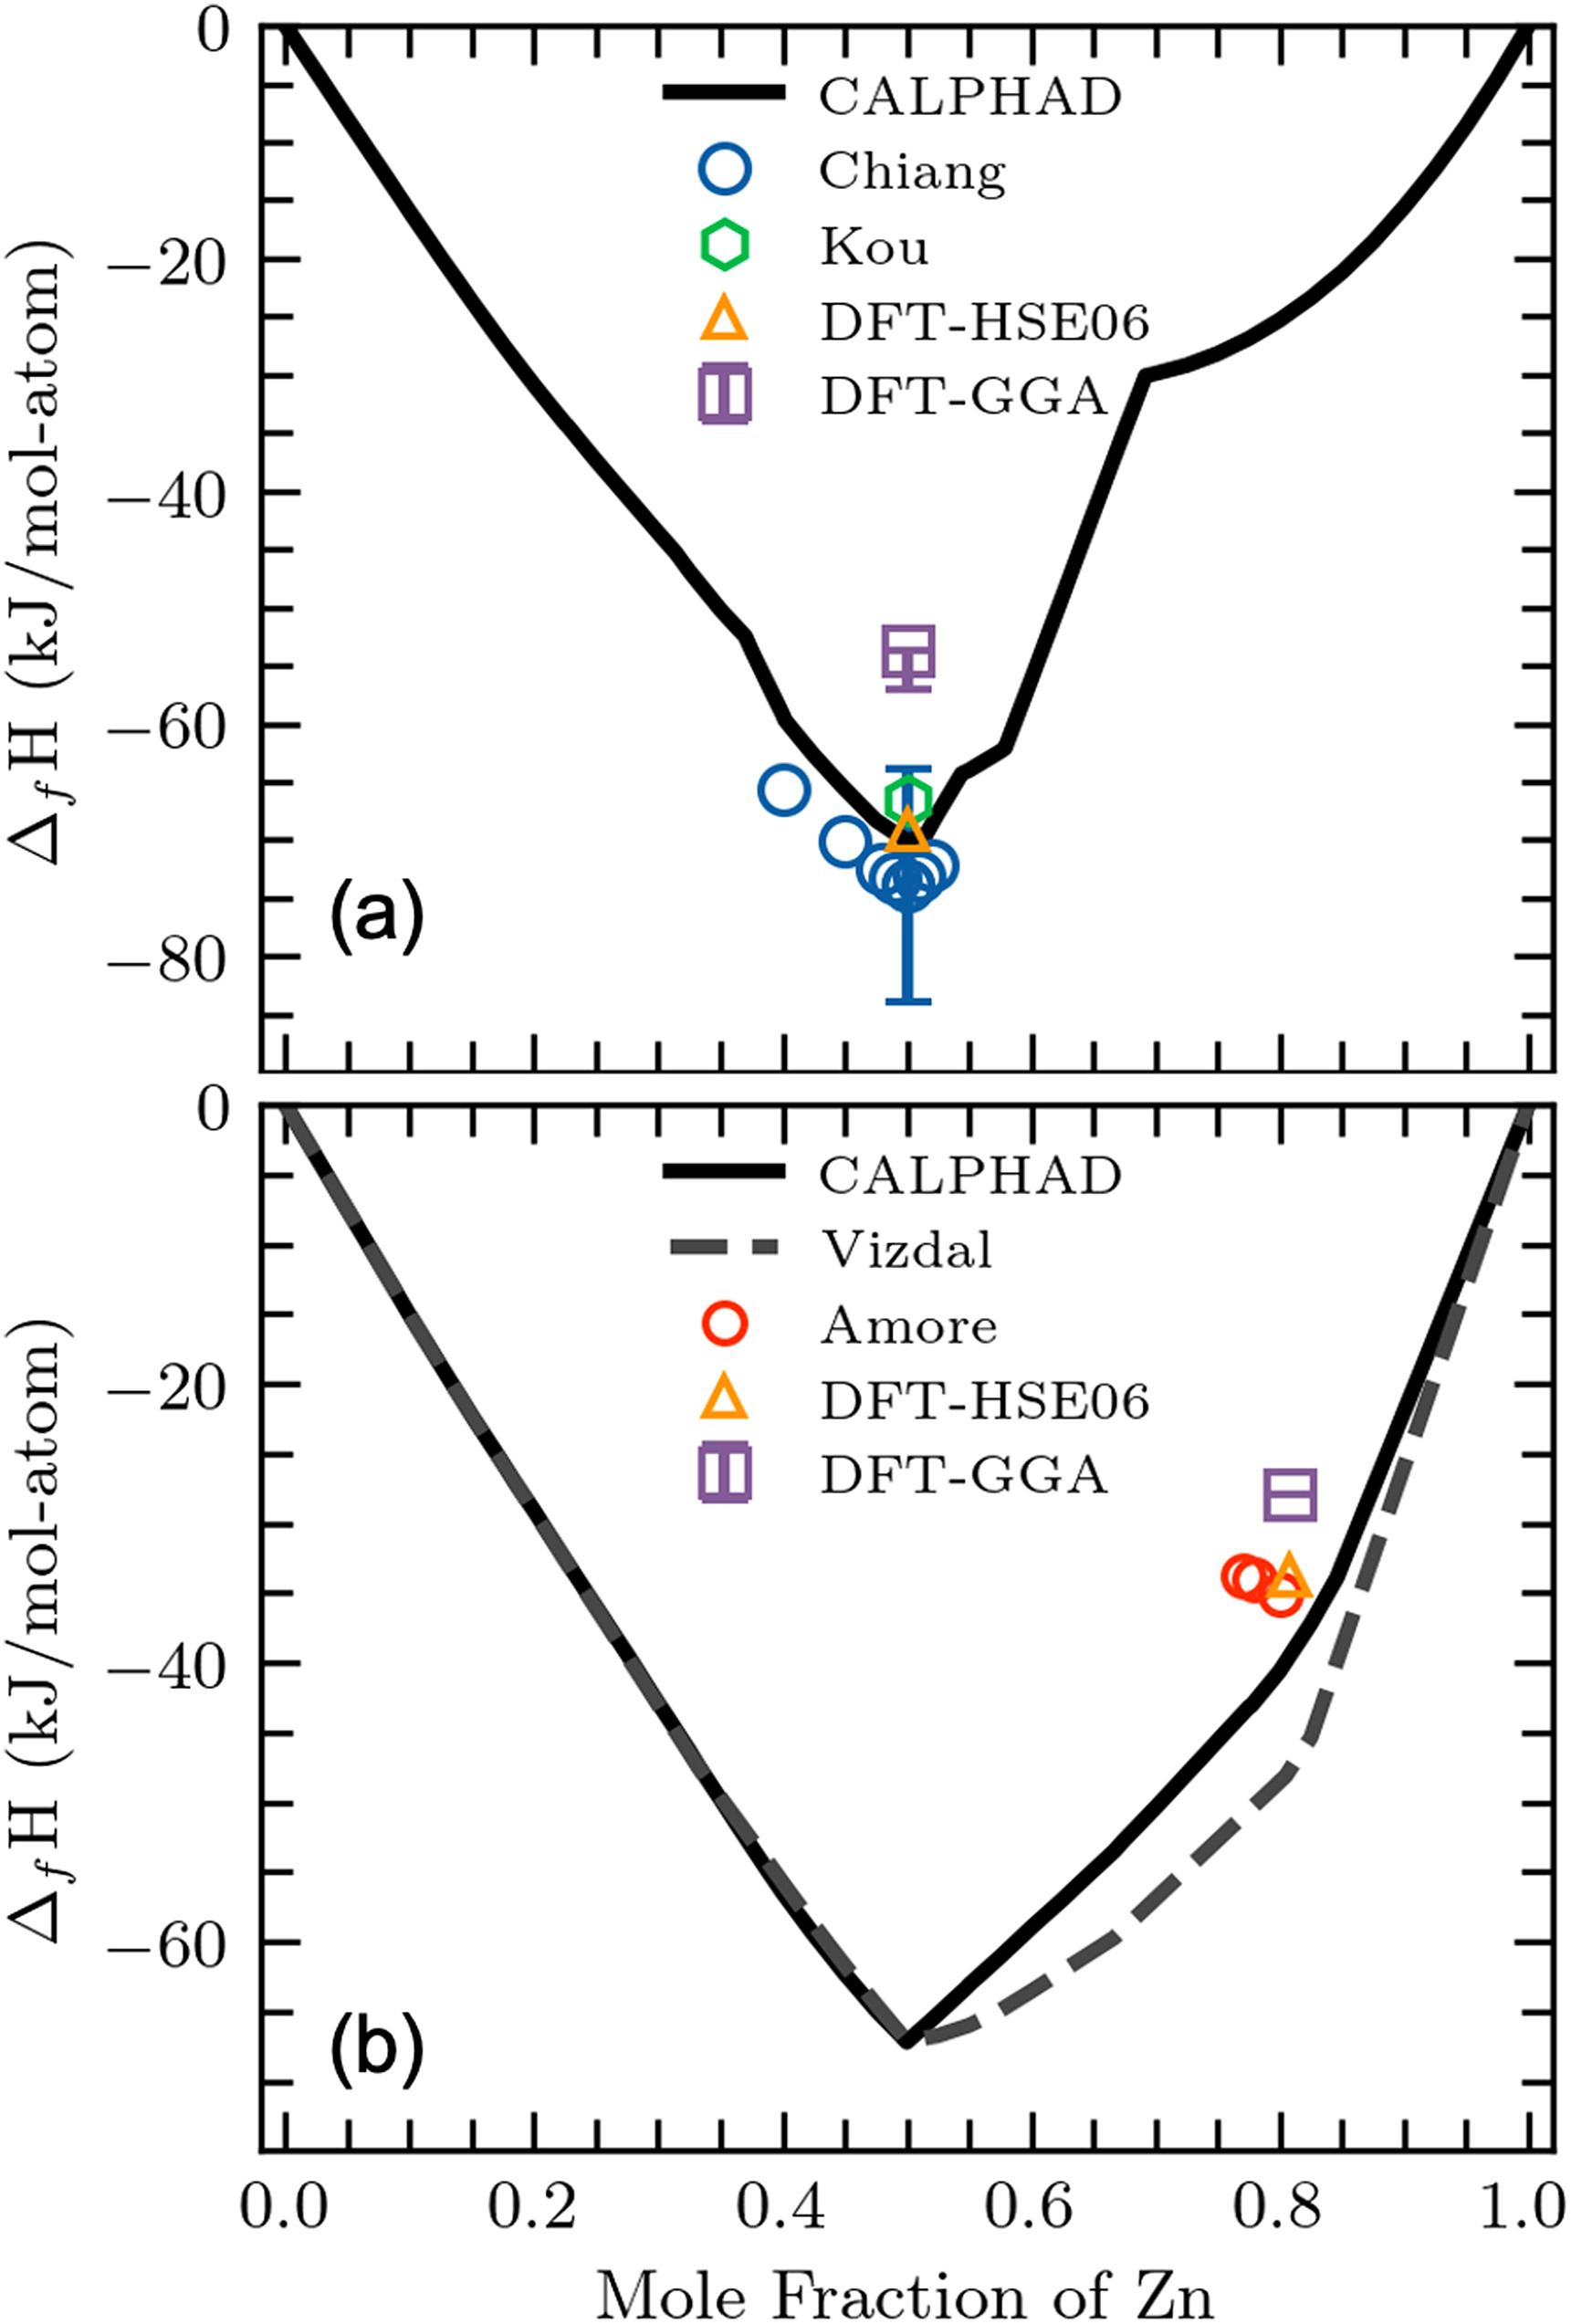
\includegraphics[width=0.5\linewidth]{intermetallics/Intermetallics-PdZnHMR.jpg}
    \caption{Calculated enthalpy of formation $\Delta_f$H at (a) 1273 K and (b) 300 K, along with DFT-based calculations and available experimental data by Chiang et al. \cite{ChiangIpserChang1977}, Kou and Chang \cite{kou1975thermodynamics}, and Amore et al. \cite{amore2009thermochemistry}. DFT using HSE is calculated at 0 K. DFT using GGA is calculated at 0 K and high temperatures 300 K and 1270 K respectively, shown as purple bars in the figure.}
    \label{intermetallics:fig:PdZnHMR}
\end{figure}

\subsection{Site occupancy in the \texorpdfstring{$\gamma$}--phase and surface construction} \label{intermetallics:ssec:PdZnsite}
Figure \ref{intermetallics:fig:PdZnSOC} shows the calculated site fractions in $\gamma$ at 773 K and 1023 K from the present model in comparison with XRD results by Edström et al. \cite{strom1969x}, Gourdon et al. \cite{gourdon2006intergrowth} and Dasgupta et al. \cite{Dasgupta2022}. Temperature has little influence on the site fraction of the $\gamma$ phase. With increasing Pd content, Pd is predicted to first occupy the OT sublattice, and then the OH sublattice after the OT sublattice is fully occupied. The site fractions of Pd in the OH sublattice are in good agreement with experimental data. For example, at $x_{Pd}$ = 0.173, the calculated site fraction of Pd in the OH sublattice $y_{Pd}^{OH}$ is 0.08, slightly higher than 0.07 measured by Dasgupta et al.\cite{Dasgupta2022} At $x_{Pd}$ = 0.181, 0.192, and 0.23, the calculated $y_{Pd}^{OH}$ values are 0.118, 0.165, and 0.333, respectively, which agree well with experimental data with a mean absolute error (MAE) of 0.002. Vizdal et al.'s \cite{vizdal2006experimental} model could not predict site fractions in $\gamma$ due to the 2-sublattice model used.

\begin{figure}[H]
    \centering
    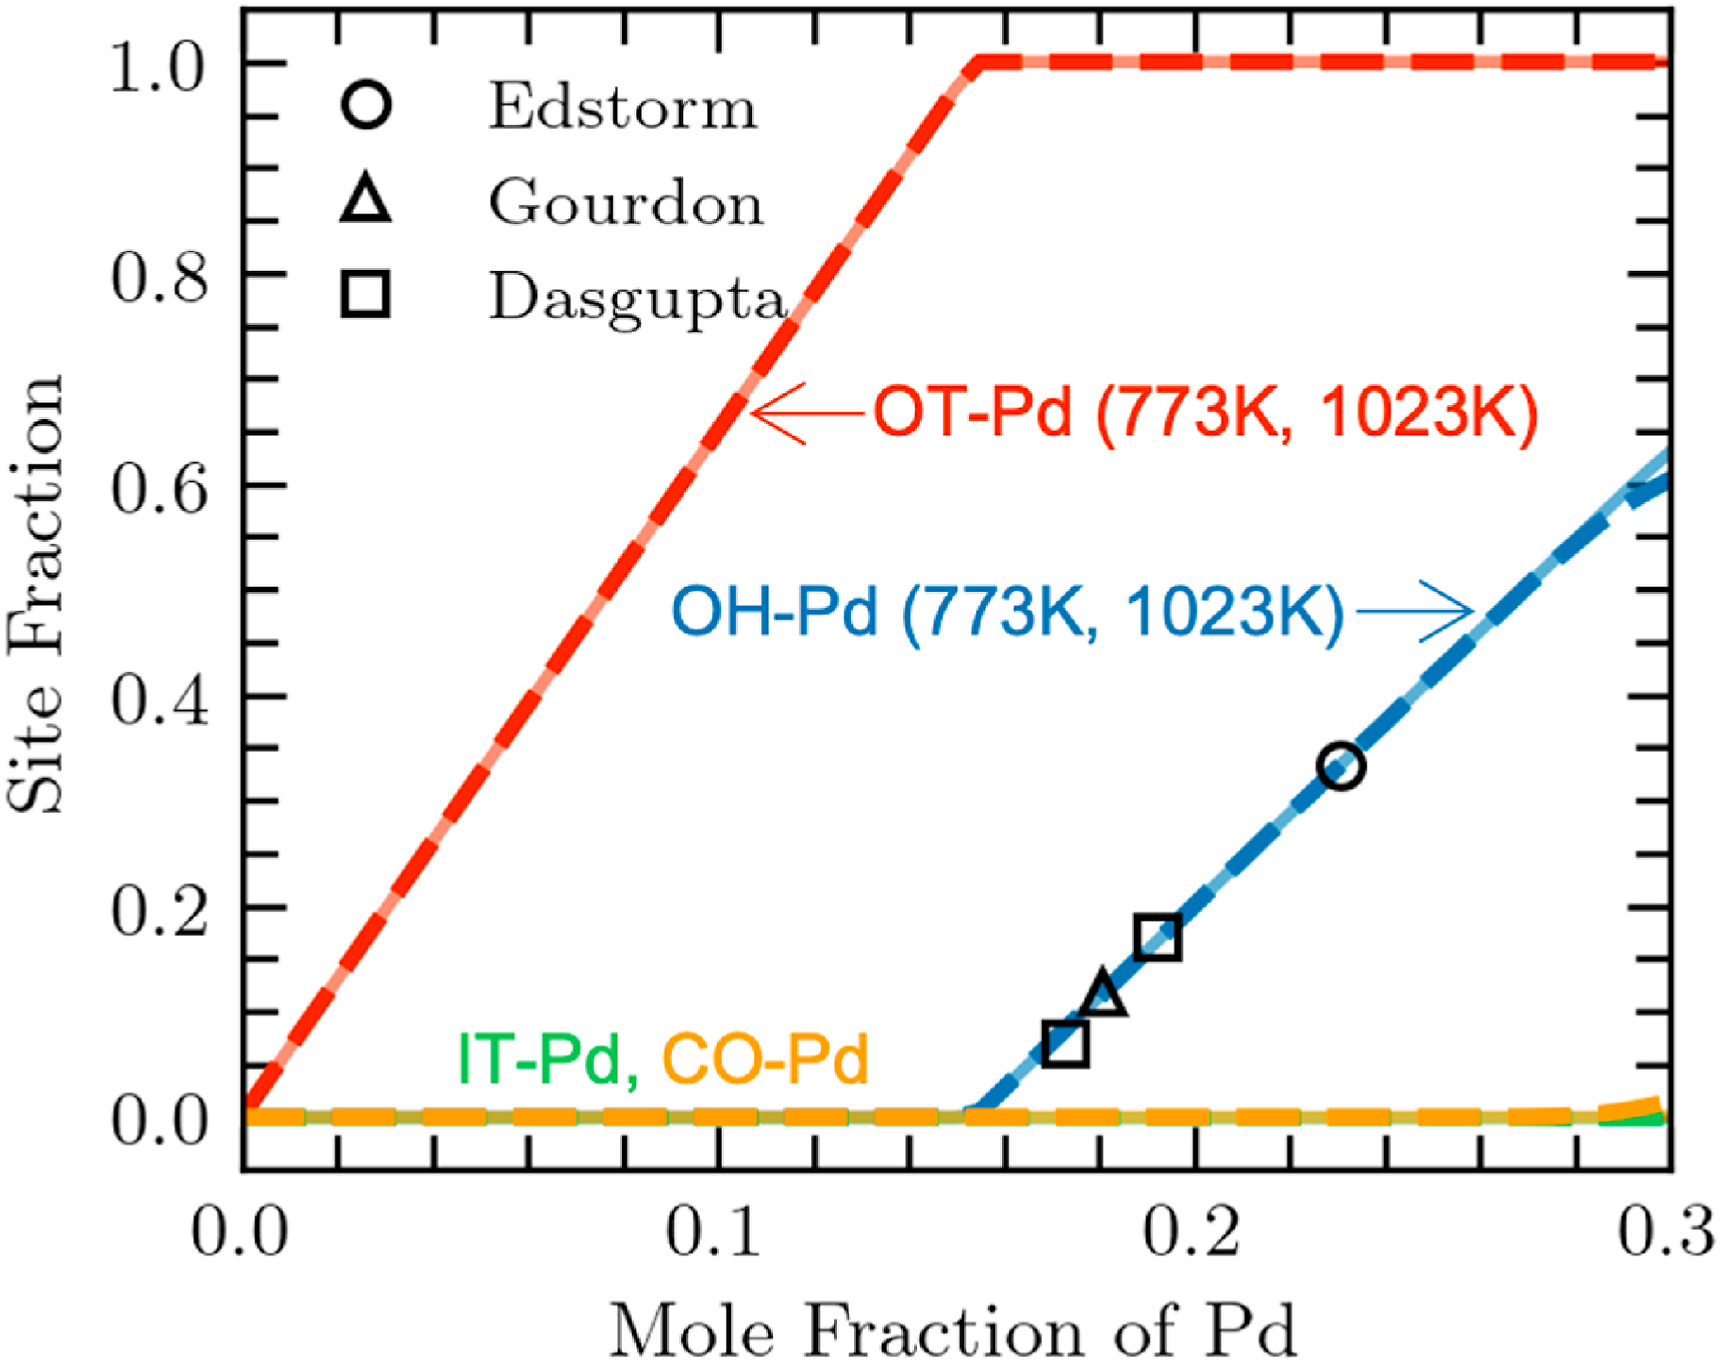
\includegraphics[width=0.5\linewidth]{intermetallics/Intermetallics-PdZnSOC.jpg}
    \caption{Calculated site fractions in $\gamma$ at 773K (solid lines) and 1023 K (dash lines) with the experimental data by Edström et al. \cite{strom1969x} at 923 K, Gourdon et al. \cite{gourdon2006intergrowth} at 1023 K, and Dasgupta et al. \cite{Dasgupta2022} at 773 K superimposed.}
    \label{intermetallics:fig:PdZnSOC}
\end{figure}

Force constants can be used to quantitatively understand interactions between atomic pairs \cite{shang2009first}. A large and positive force constant suggests a strong bonding interaction of an atomic pair, whereas a negative force constant indicates the tendency to separate \cite{yu2019synthesis}. To understand the site occupancy of Pd in $\gamma$, we examined energies and force constants in three Pd$_9$Zn$_{43}$ configurations to analyze the occupancy of an additional Pd atom compared to the full Pd OT occupation in Pd$_8$Zn$_{44}$. Three configurations are $({{\rm Pd}_8)}^{OT}{{(\rm Pd}_1{\rm Zn}_{11})}^{OH}({{\rm Zn}_8)}^{IT}({{\rm Zn}_{24})}^{CO}$, \\$({{\rm Pd}_8)}^{OT}{({\rm Zn}_{12})}^{OH}({{{\rm Pd}_1\rm Zn}_7)}^{IT}({{\rm Zn}_{24})}^{CO}$, and $({{\rm Pd}_8)}^{OT}{({\rm Zn}_{12})}^{OH}({{\rm Zn}_8)}^{IT}({{{\rm Pd}_1\rm Zn}_{23})}^{CO}$, where 8 Pd atoms occupy 8 OT sites and the 9th Pd atom occupies one of the OH (conf\_OH), IT (conf\_IT), or CO (conf\_CO) sites, respectively. Force constants can be predicted by DFT-based phonon calculations \cite{shang2018understanding}. Table \ref{intermetallics:PdZn_DFT_details} lists details of phonon calculations for Pd$_9$Zn$_{43}$ configurations. Figure \ref{intermetallics:fig:PdZnFC} shows the force constants of atomic pairs Pd-Pd, Pd-Zn, and Zn-Zn in three Pd$_9$Zn$_{43}$ configurations. The Pd-Zn atomic pairs have the largest force constants 5.373 eV/\r{A}$^2$, compared with 4.875 eV/\r{A}$^2$ of Pd-Pd and 3.569 eV/\r{A}$^2$ of Zn-Zn pairs. It indicates that Pd-Zn pairs have the strongest bonding in the configuration. Table \ref{intermetallics:tab:PdZnfc} shows the energy and bonding in three Pd$_9$Zn$_{43}$ configurations, i.e., conf\_OH, conf\_IT, and conf\_CO. conf\_OH has the lowest energy $E_{conf\_OH}$ = -105.30 eV/atom and the shortest Pd-Zn bonding distance d$_{conf\_OH}^{Pd-Zn}$ = 2.538 \r{A} in comparison with conf\_CO and conf\_IT. In contrast, $d_{conf\_OH}^{Pd-Pd}$ = 2.940 \r{A} is larger than that of conf\_OH and conf\_IT. Table \ref{intermetallics:tab:PdZnfc} also shows the bonding of the 9th Pd when occupying OH, CO, and IT. In conf\_OH, the 9th Pd is bonding with Zn atoms in its first nearest neighbors ($d^{1NN}$ < 3.2 \r{A}, seen in Figure \ref{intermetallics:fig:PdZnFC}), with the nearest Pd atom is 4.713 \r{A} away. In conf\_CO and conf\_IT, there are Pd-Pd pairs in the first nearest neighbors of the 9th Pd, which makes the bonding between Pd and surroundings weaker than that in conf\_OH. We conclude that the stability preference for OH occupancy of additional Pd atoms results from stronger Pd-Zn bonding interactions.

\begin{figure}[H]
    \centering
    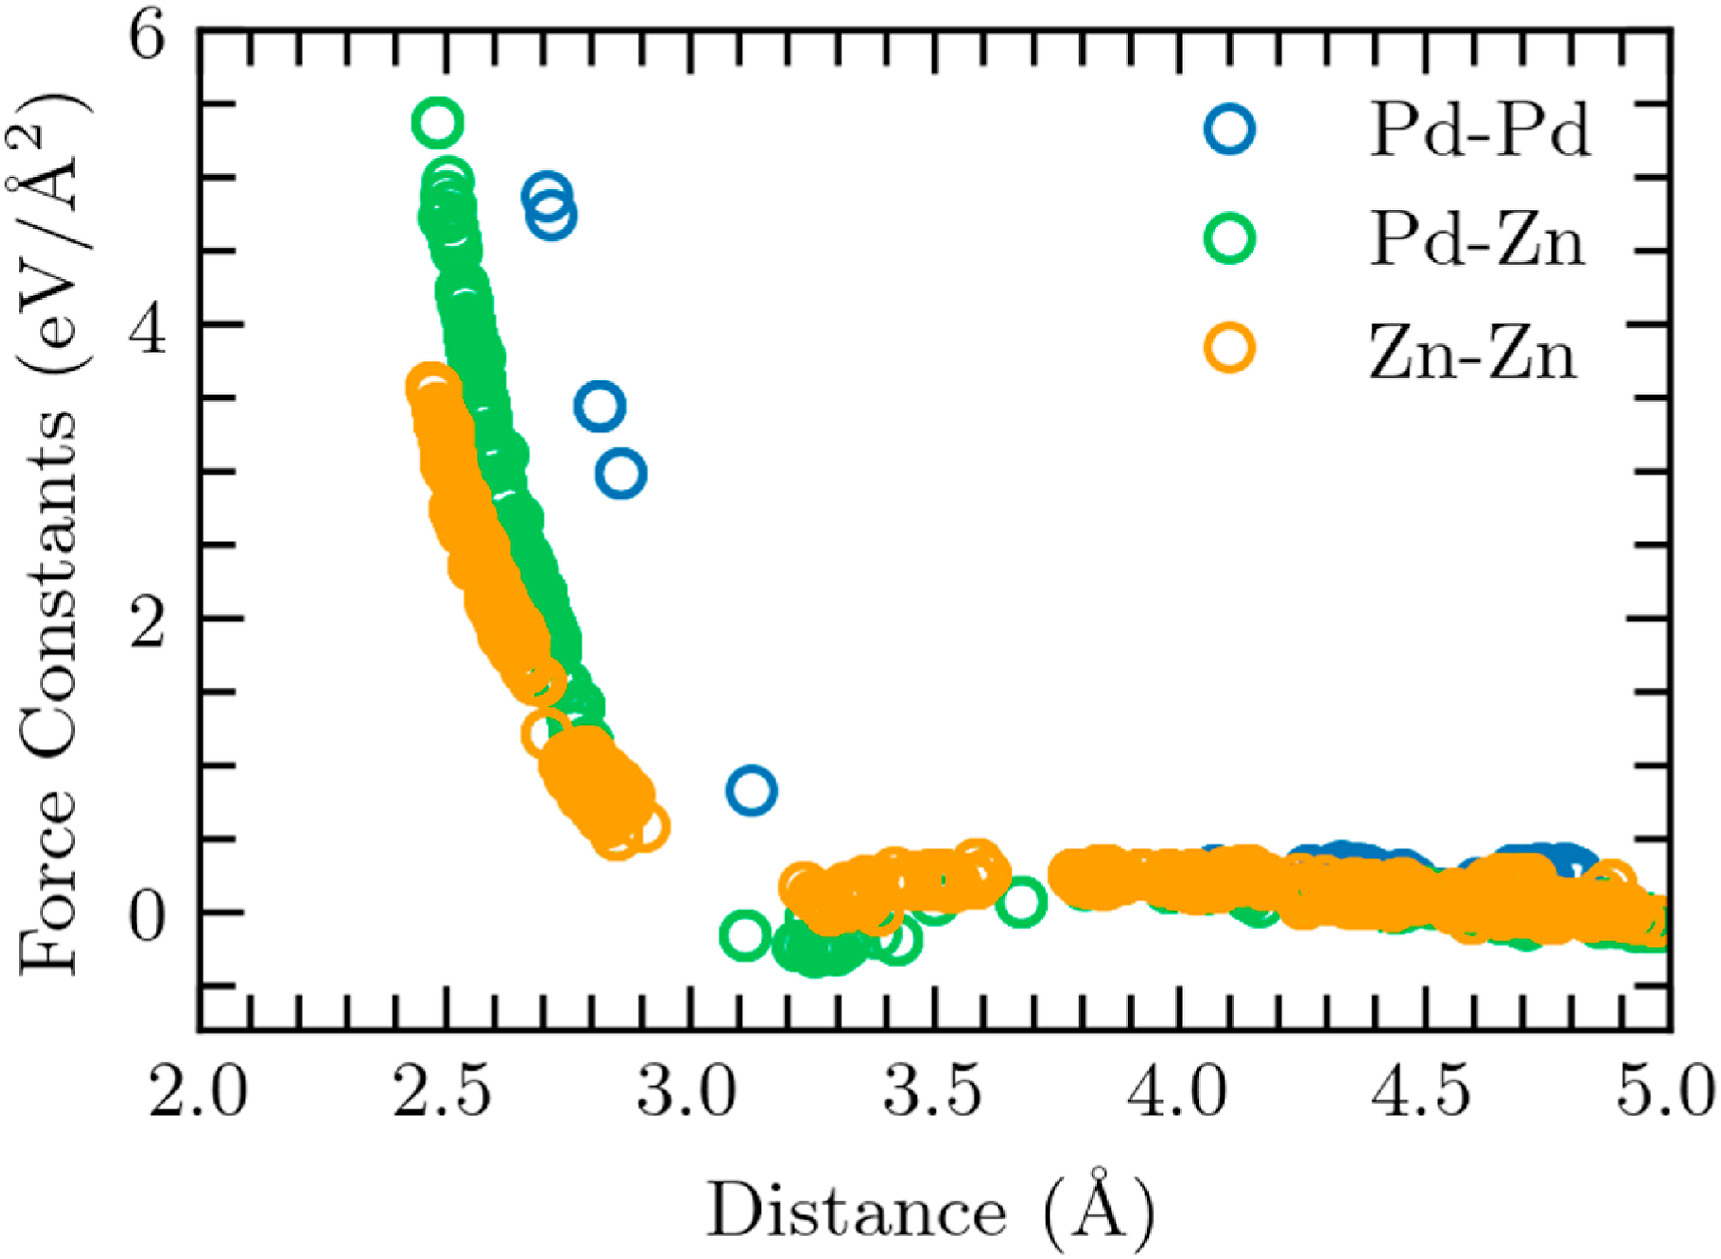
\includegraphics[width=0.5\linewidth]{intermetallics/Intermetallics-PdZnFC.jpg}
    \caption{Force constants of Pd-Pd, Pd-Zn, and Zn-Zn atom pairs in Pd9Zn43 configurations obtained from phonon calculations.}
    \label{intermetallics:fig:PdZnFC}
\end{figure}

\begin{table}[H]
    \centering
    \caption{Energies, and distances of bonds (d) of the nearest pairs for three Pd$_9$Zn$_{43}$ configurations with the first 8 Pd atoms occupying the OT site, and the 9th Pd atom (Pd$^{9th}$) occupying the OH, CO, or IT site, denoted by conf\_OH, conf\_CO, and conf\_IT, respectively. Configurations are relaxed using DFT calculations.}
    \begin{tabular}{>{\raggedright\arraybackslash}m{3cm}>{\raggedright\arraybackslash}m{3cm}>{\raggedright\arraybackslash}m{2cm}>{\raggedright\arraybackslash}m{2cm}>{\raggedright\arraybackslash}m{2.5cm}>{\raggedright\arraybackslash}m{2.5cm}}
        \hline
         \textbf{Configurations}& \textbf{Energy (eV/atom)} & d of Pd-Zn (\r{A}) & d of Pd-Pd (\r{A}) & d of Pd$^{9th}$-Zn (\r{A}) & d of Pd$^{9th}$-Pd (\r{A})\\
        \hline
        conf\_OH&-105.30&2.538&2.940&2.563&4.713\\
        conf\_CO&-104.89&2.558&2.783&2.562&2.783\\
        conf\_IT&-104.74&2.560&2.887&2.613&3.192\\
         \hline
    \end{tabular}
    \label{intermetallics:tab:PdZnfc}
\end{table}

Site fractions of $\gamma$ phase calculated from the CALPHAD modeling are further applied to analyze the surface structures. The possible stable composition of the $\gamma$ phase is evaluated ranging from Pd$_8$Zn$_{44}$ to Pd$_{12}$Zn$_{40}$ from the present model. It indicates that site occupancy in OH will be changed with changing Pd composition in the $\gamma$ phase, with OT remaining occupied by Pd, IT and CO occupied by Zn. DFT-based calculations have suggested that the $(1\bar{1}0)$ surface of the $\gamma$ phase has a lower surface energy than $(110)$ and ${111}$ \cite{Dasgupta2022}. Figure \ref{intermetallics:fig:PdZnSurface} shows $(1\bar{1}0)$ surface constructions of $\gamma$ phase. OT sites separately locate on the surface, forming Pd monomers (Pd1). When increase Pd occupy OH sites, OT-OH-OT ensembles on the surface can then become Pd trimers (Pd3). The ability to control the exposure of specific surface ensembles between Pd1 and Pd3 sites is a direct consequence of the site occupancies of the bulk structure and has catalytic consequences. For example, the activity for ethylene hydrogenation and selectivity for acetylene semi-hydrogenation were drastically altered by tuning active ensembles between Pd monomers (Pd1) and Pd trimers (Pd3) \cite{Dasgupta2022}. 

\begin{figure}[H]
    \centering
    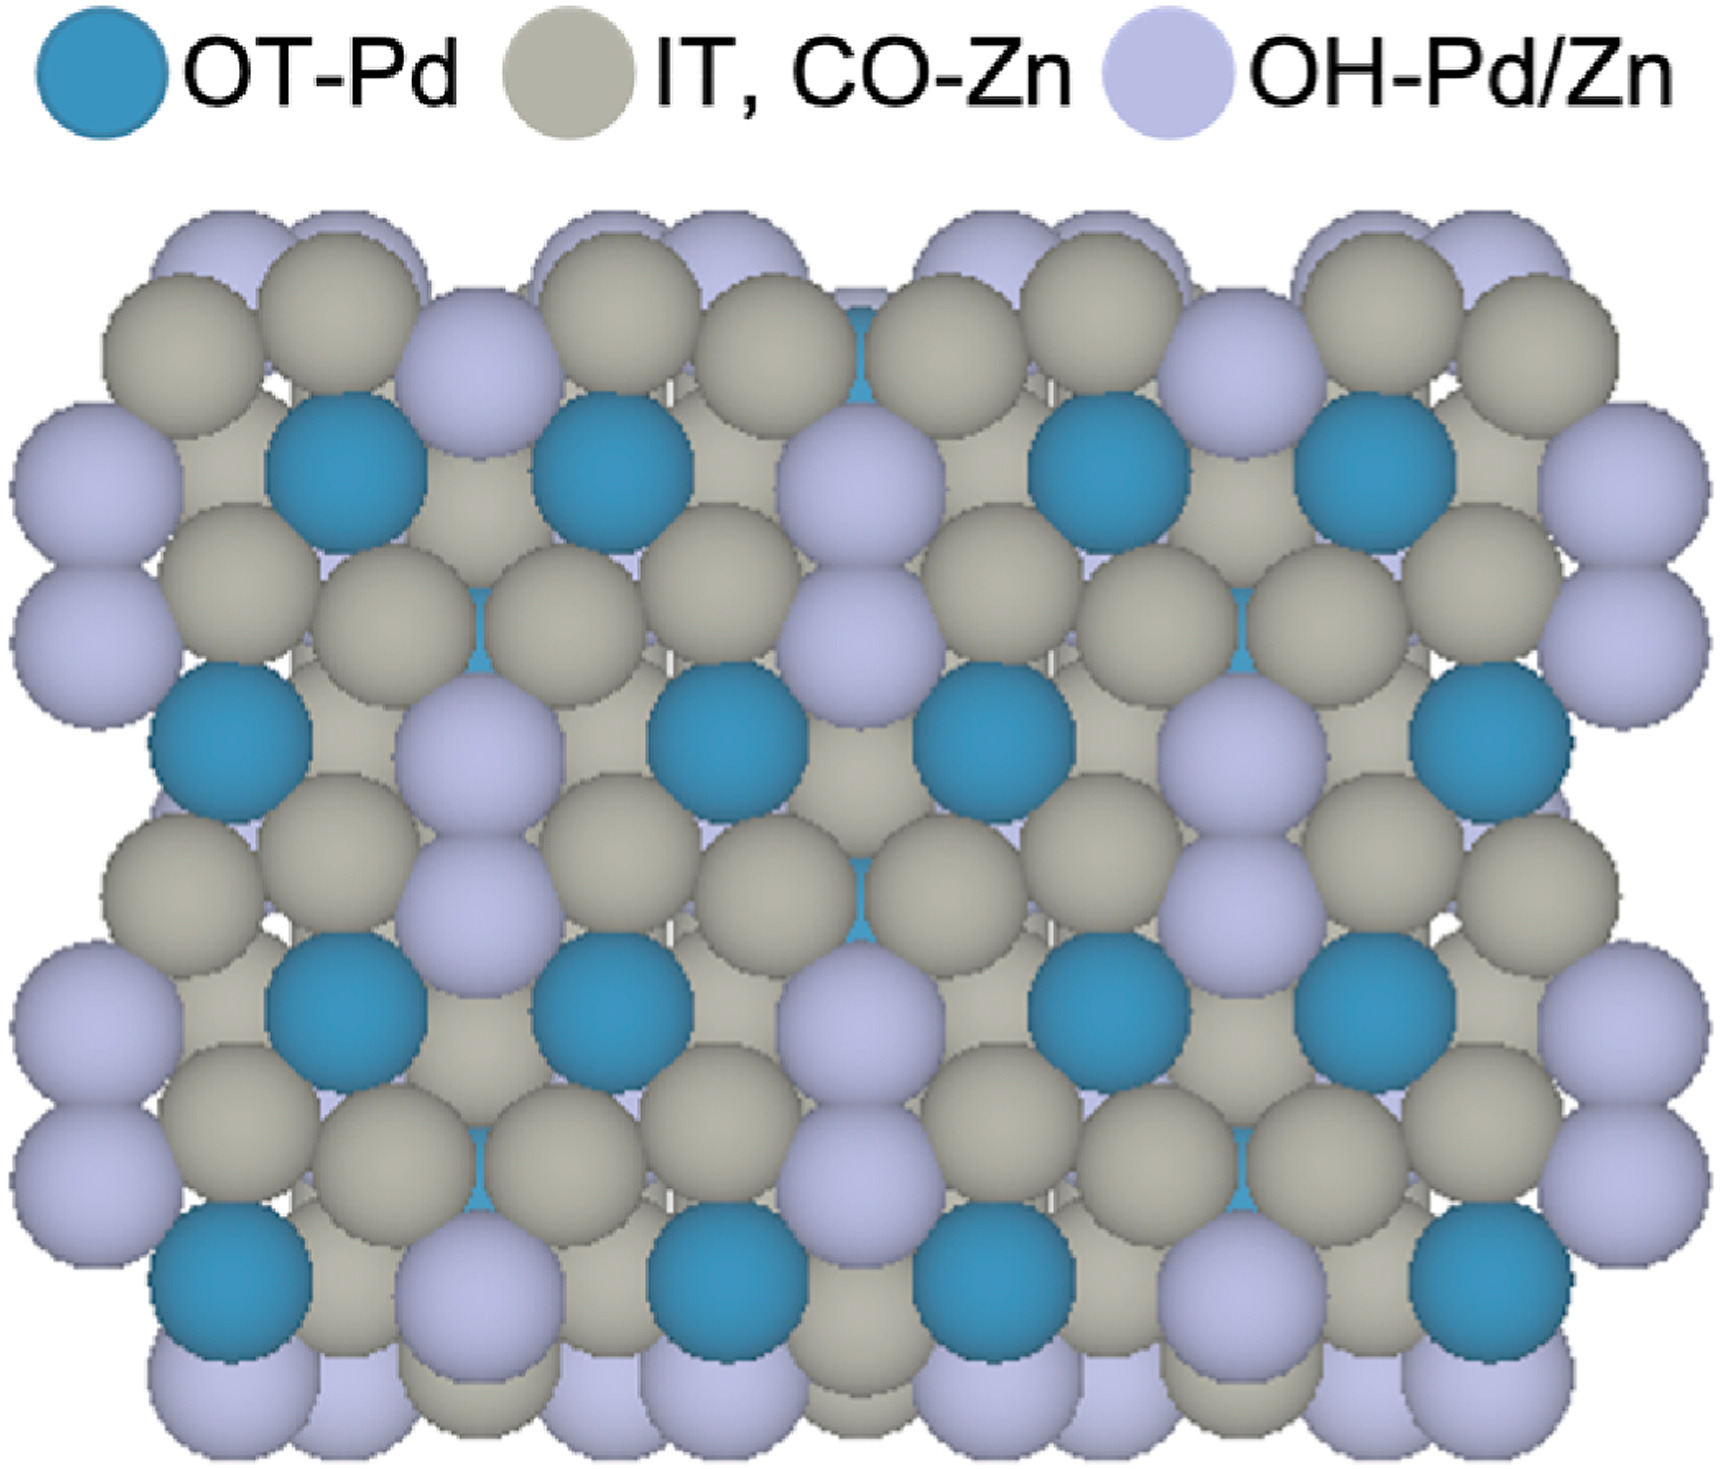
\includegraphics[width=0.4\linewidth]{intermetallics/Intermetallics-PdZnSurface.jpg}
    \caption{$(1\bar{1}0)$ surface of $\gamma$ in $2\times2\times2$ supercell. Blue atoms are OT sites, which are occupied by Pd atoms. Grey atoms are IT and CO sites, which are occupied by Zn atoms. Purple atoms are OH sites, which can be occupied by both Pd and Zn atoms.}
    \label{intermetallics:fig:PdZnSurface}
\end{figure}

\section{Determination of site occupancy in the M-Pd-Zn (M = Cu, Ag, and Au) \texorpdfstring{$\gamma$}--brass phase} \label{intermetallics:sec:PdZnM}







\subsection{Literature review} \label{intermetallics:ssec:PdZnMlit}


\subsection{Modeling details} \label{intermetallics:ssec:PdZnMmodel}


\subsection{Results and discussion} \label{intermetallics:ssec:PdZnMresult}


\section{Summary} \label{intermetallics:sec:Summary}
%%% Pd-Zn Binary
Thermodynamic modeling of the Pd-Zn system based on the CALPHAD approach has been performed with thermochemical and phase equilibria data from experiments in the literature and DFT-based total energy and phonon calculations in the present work. A 4-sublattice model is used to describe the $\gamma$ phase in accordance with its four Wyckoff positions providing a better prediction of surface construction and enabling the understanding of active surface ensembles for catalysts. DFT-based first-principles calculations are used to obtain Gibbs energies of endmembers for the $\gamma$ phase. High throughput CALPHAD modeling tools (i.e., ESPEI and PyCalphad) are employed to evaluate model parameters. Uncertainty of activity is quantified in the present work. In the $\gamma$ phase, Pd atoms first occupy the OT sublattice followed by the OH sublattice, as indicated by DFT-based total energy and phonon calculations supported by the bonding distance and force constants analyses and in agreement with experimental data. Site fractions calculated from the CALPHAD modeling as a function of temperature and composition contribute to analyzing surface construction of the $\gamma$ phase. It further improves tailoring and understanding of active ensembles on the surface and enhances catalytic performance.

%%% Pd-Zn-M Ternary

%%% Model